 % ============================================================================
%  The Legend Challenge: Embedding Ethical Compliance into LLMs through Champion
%  Narratives in the Gender Equality Domain
%  ---------------------------------------------------------------------------
%  Generated by following paper_plan.md (Section Blueprint §4) and pipeline.md.
%  Sections 1 (Introduction) and 2 (Related Work) are intentionally left as
%  \input{} placeholders; the corresponding .tex files exist as separate drafts
%  (paper_draft_abstract_intro.md, paper_draft_related_work.md). Methodology
%  onward is drafted in full below.
% ============================================================================

\documentclass[pdflatex, sn-apa]{sn-jnl}% Math and Physical Sciences

\usepackage{graphicx}%
\usepackage{multirow}%
\usepackage{amsmath,amssymb,amsfonts}%
\usepackage{amsthm}%
\usepackage{mathrsfs}%
\usepackage[title]{appendix}%
\usepackage{xcolor}%
\usepackage{textcomp}%
\usepackage{manyfoot}%
\usepackage{booktabs}%
\usepackage{algorithm}%
\usepackage{algorithmicx}%
\usepackage{algpseudocode}%
\usepackage{listings}%
%%%%


%% as per the requirement new theorem styles can be included as shown below
\theoremstyle{thmstyleone}%
\newtheorem{theorem}{Theorem}%  meant for continuous numbers
%%\newtheorem{theorem}{Theorem}[section]% meant for sectionwise numbers %
%optional argument [theorem] produces theorem numbering sequence instead of
%independent numbers for Proposition
\newtheorem{proposition}[theorem]{Proposition}% 
%%\newtheorem{proposition}{Proposition}% to get separate numbers for theorem and
%proposition etc.

\theoremstyle{thmstyletwo}%
\newtheorem{example}{Example}%
\newtheorem{remark}{Remark}%

\theoremstyle{thmstylethree}%
\newtheorem{definition}{Definition}%

\raggedbottom
%%\unnumbered% uncomment this for unnumbered level heads


% ---------- Packages --------------------------------------------------------
\usepackage[T1]{fontenc}
\usepackage[utf8]{inputenc}
\usepackage[english]{babel}
\usepackage[expansion=false]{microtype}
\usepackage{geometry}
\geometry{margin=1in}

\usepackage{booktabs}      % Professional table rules
\usepackage{tabularx}      % Flexible tables
\usepackage{array}
\usepackage{multirow}
\usepackage{colortbl}
\usepackage{makecell}

\usepackage{graphicx}
\usepackage{caption}
\usepackage{subcaption}
\usepackage{float}
\usepackage{placeins}

\usepackage{amsmath, amssymb, amsfonts}
\usepackage{mathtools}

\usepackage{pgfplots}
\pgfplotsset{compat=1.18}

\usepackage{xcolor}
\usepackage{hyperref}
\hypersetup{ colorlinks=true, linkcolor=black!50!blue, citecolor=black!50!blue,
  urlcolor=black!50!blue, }
\usepackage[noabbrev]{cleveref}

% Tell cleveref what to call lstlisting environments
\crefname{lstlisting}{listing}{listings}
\Crefname{lstlisting}{Listing}{Listings}

\usepackage{listings}
\usepackage{tcolorbox}
\tcbuselibrary{listings, breakable, skins}

\usepackage{enumitem}
\setlist{nosep, leftmargin=1.25em}
% ---------- Result-highlight macros (from paper-writing/assets/table-style.tex)
\definecolor{bestred}{HTML}{B22222}
\definecolor{secondblue}{HTML}{1F3A8A}
\definecolor{gaingreen}{HTML}{006400}
\definecolor{boxbg}{HTML}{F5F5F5}
\newcommand{\best}[1]{\textcolor{bestred}{\textbf{#1}}}
\newcommand{\second}[1]{\textcolor{secondblue}{\underline{#1}}}
\newcommand{\gain}[1]{\textcolor{gaingreen}{#1}}

% ---------- Listings style for JSON / prompt snippets ----------------------
\lstdefinelanguage{json}{ basicstyle=\ttfamily\footnotesize,
  showstringspaces=false, breaklines=true, frame=none, literate=
  *{0}{{{\color{black!60}0}}}{1} {1}{{{\color{black!60}1}}}{1}
  {2}{{{\color{black!60}2}}}{1} {3}{{{\color{black!60}3}}}{1}
  {4}{{{\color{black!60}4}}}{1} {5}{{{\color{black!60}5}}}{1}
  {6}{{{\color{black!60}6}}}{1} {7}{{{\color{black!60}7}}}{1}
  {8}{{{\color{black!60}8}}}{1} {9}{{{\color{black!60}9}}}{1}, } \lstset{
  basicstyle=\ttfamily\footnotesize, breaklines=true, columns=fullflexible,
  showstringspaces=false, }

\newtcolorbox{promptbox}[1][]{ colback=boxbg, colframe=black!40,
  fonttitle=\bfseries, breakable, sharp corners, boxrule=0.4pt, left=4pt,
  right=4pt, top=4pt, bottom=4pt, #1 }

% ---------- Custom macros --------------------------------------------------
\newcommand{\modelbase}{\texttt{base}}
\newcommand{\modellegends}{\texttt{tuned-legends}}
\newcommand{\modelreg}{\texttt{tuned-regulation}}
\newcommand{\bm}{\textbf}



\begin{document}

\title[The Legend Challenge: Embedding Ethical Compliance into LLMs through Champion Narratives in the Gender Equality Domain]{The Legend Challenge: Embedding Ethical Compliance into LLMs through Champion Narratives in the Gender Equality Domain}

\author*[1]{\fnm{Fatmir} \sur{Bylyshi}}\email{fatmir.bylyshi@studenti.unimi.it}
\equalcont{These authors contributed equally to this work.}

\author*[1]{\fnm{El-Khazri} \sur{Hicham}}\email{hicham.elkhazri@studenti.unimi.it}
\equalcont{These authors contributed equally to this work.}

\author*[1]{\fnm{Ouardi} \sur{Ilyass}}\email{ilyass.ouardi@studenti.unimi.it}
\equalcont{These authors contributed equally to this work.}

\affil*[1]{\orgdiv{Department of Computer Science}, \orgname{University of
Milan}, \orgaddress{\street{Via Celoria, 20}, \city{Milan},
\postcode{20134}, \country{Italy}}}

%%==================================%%
%% Sample for unstructured abstract %%
%%==================================%%

\abstract{\citet{sargsyan2025legends} proposed that fine-tuning large language
models on \emph{legends} (synthetic narrative exemplars of compliant behaviour)
may embed regulatory ethics more effectively than fine-tuning on the underlying
regulatory text, but provided neither an empirical verification nor a
measurement instrument. We provide both. We compare legend-based fine-tuning
with regulation-text-based fine-tuning on a single regulation (the EU Gender
Equality Strategy 2020--2025) and a single backbone
(\texttt{gpt-4o-2024-08-06}), holding the system prompt, the training format and
the JSONL line count constant, so that corpus content is the only experimental
variable. To make the comparison measurable we introduce \textbf{GenderEqGLUE},
a five-task benchmark: GE-CLS, GE-NLI, GE-QA, GE-WSC and GE-NEXT, adapted
one-to-one from the GLUE and SuperGLUE templates. To examine \emph{how} each
model arrives at its predictions we conduct an interpretability analysis based
on the log-probabilities exposed by the OpenAI API for the fine-tuned models,
measuring via \textbf{structured occlusion} how much each model depends on the
scenario and on the regulatory clause over a stratified sample of 60 GE-NLI
items. The analysis shows that both fine-tuned variants sharply reduce their
dependence on explicit context relative to the unadapted model, and that
\modellegends{} depends on the regulatory clause almost three times more than
\modelreg{} ($p = 0.0001$), with the divergence concentrated on the decidable
labels and absent on \texttt{neutral}. On the aggregate GenderEqGLUE Score,
\modelreg{} leads with 0.938, \modellegends{} follows with 0.926 and
\modelbase{} comes last with 0.904; per-task wins split 3--3 between the two
fine-tuning regimes (\modelbase{} wins none). \modellegends{} is the strongest
model on the task that is central to the hypothesis, compliant-action selection,
GE-NEXT. The two regimes therefore teach \textbf{complementary competences}:
legends teach compliance recognition and compliant-action selection; the
regulatory text teaches ontology recognition and factual recall of short text
spans. The deployment choice should be driven by the application's dominant risk
profile.}

\maketitle
% ============================================================================
%  §1 — INTRODUCTION
% ============================================================================
\section{Introduction}
\label{sec:intro}
 
\begin{figure}[t]
\centering
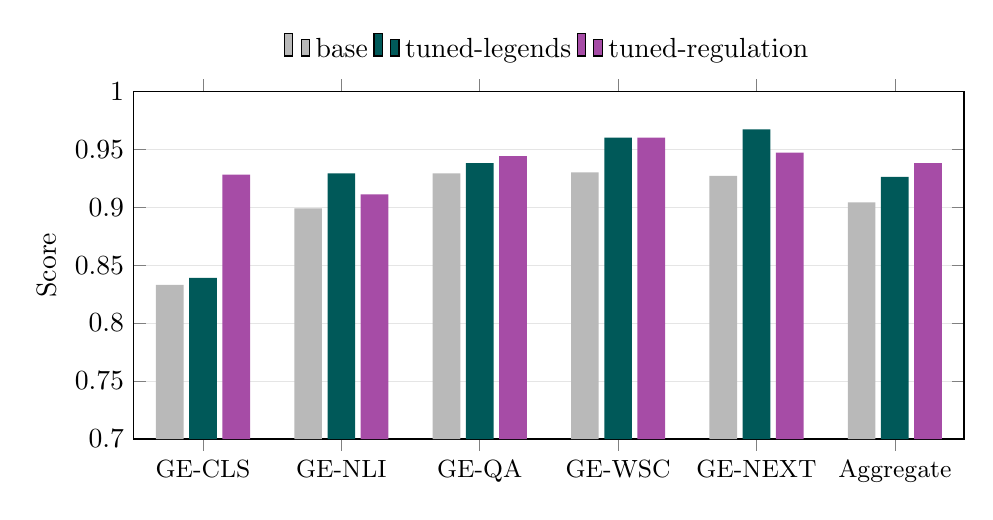
\begin{tikzpicture}
\begin{axis}[ ybar, width=\linewidth, height=6cm, bar width=10pt, ymin=0.70,
    ymax=1.0, ylabel={Score}, ytick={0.70,0.75,0.80,0.85,0.90,0.95,1.0},
    symbolic x coords={GE-CLS,GE-NLI,GE-QA,GE-WSC,GE-NEXT,Aggregate},
    xtick=data, x tick label style={font=\small}, legend style={at={(0.5,1.05)},
    anchor=south, legend columns=3, draw=none}, enlarge x limits=0.10,
    ymajorgrids, major grid style={gray!20}, ] \addplot[fill=gray!55,draw=none]
    coordinates
    {(GE-CLS,0.833)(GE-NLI,0.899)(GE-QA,0.929)(GE-WSC,0.930)(GE-NEXT,0.927)(Aggregate,0.904)};
    \addplot[fill=teal!70!black,draw=none] coordinates
    {(GE-CLS,0.839)(GE-NLI,0.929)(GE-QA,0.938)(GE-WSC,0.960)(GE-NEXT,0.967)(Aggregate,0.926)};
    \addplot[fill=violet!70,draw=none] coordinates
    {(GE-CLS,0.928)(GE-NLI,0.911)(GE-QA,0.944)(GE-WSC,0.960)(GE-NEXT,0.947)(Aggregate,0.938)};
\legend{base, tuned-legends, tuned-regulation}
\end{axis}
\end{tikzpicture}
\caption{The two fine-tuning regimes teach complementary competences.
\modelreg{} leads on the aggregate score; \modellegends{} is the strongest
model on GE-NEXT and GE-NLI.}
\label{fig:teaser}
\end{figure}
 
% ¶1 — Task: regulatory complexity → AI as compliance tool → paradox

\paragraph{Regulatory complexity and AI as a compliance instrument}
The contemporary regulatory landscape for sustainability is extremely complex;
as~\citet{sargsyan2025legends} observe, it is characterised by overlapping
requirements, policy gaps and a consequent rapid expansion of new rules. The
Corporate Sustainability Reporting Directive requires large firms to report on
social matters, including gender equality
policies~\citep{europeancommission2022csrd}; the EU Taxonomy Regulation obliges
financial institutions to declare alignment
percentages~\citep{europeancommission2025taxonomy}; the Women on Boards
Directive imposes representation targets for the underrepresented gender on the
boards of listed companies~\citep{europeanparliament2022wob}; and the Pay
Transparency Directive establishes wage-transparency reporting
obligations~\citep{europeancommission2025equalpay}. Superimposed on these public
obligations are the internal policies that individual firms maintain on ethics,
diversity and inclusion, all of which must be weighed in any single corporate
decision~\citep{sargsyan2025legends}. Generative AI is widely proposed as an
instrument for translating sustainability requirements into operational
decisions~\citep{storey2025genai}, yet the optimisation objective these models
inherit is structurally narrow: cost reduction and profit maximisation.
 
% ¶2 — Challenge: the compliance paradox
\paragraph{The compliance paradox}
\citet{sargsyan2025legends} formalise this tension as the \emph{compliance
paradox}: when practical implementation is driven exclusively by profit
maximisation, a conflict with regulatory intent arises. Their canonical
illustration is a hiring scenario in which a firm committed to gender equality
adopts a Human Resource Management module that, although designed to be
``gender-blind'', favours a male candidate whose profile satisfies only 80\% of
the stated requirements. The optimisation-driven decision contradicts both the
firm's declared commitment and the underlying regulatory expectation.
\citet{sargsyan2025legends} further locate the implementation pressure point of
this paradox at the level of middle management: ``Critically, the direct
implementation of policies and regulations by middle management and their
potential focus on costs and profits creates a conflict of interest when AI
implementation is delegated to them''. The structural diagnosis is that middle
managers, charged with operationalising both regulatory directives and corporate
strategy, may rationally prioritise the cost objective---the one on which their
performance is measured---over regulatory directives, whose enforcement is remote
and probabilistic. The fact that by 2026 twenty per cent of organisations will
use AI to halve middle-management roles~\citep{economist2024gartner} only
intensifies this tension, because the layer most exposed to
regulation-versus-cost arbitrage is also the one most exposed to replacement by
AI.

% ¶3 — Prior approaches and their limitations
\paragraph{Prior approaches and their limitations}
Two responses to this paradox appear in the literature. The first is
\emph{ex~post}: firms make decisions independently and regulatory compliance is
assessed after the fact. \citet{sargsyan2025legends} argue that reactive delay is
unacceptable for high-impact social outcomes. The second is \emph{ex~ante}:
regulatory considerations are embedded directly into the AI system, for example
through contextual regulatory alignment~\citep{achintalwar2024alignment} or
machine-readable semantic formats~\citep{mclaughlin2021x2rl}. These approaches
require translating the regulation into a formal representation, a process whose
difficulty across jurisdictions, languages and sources of authority is repeatedly
reported in the digital-ready legislation
literature~\citep{motzfeldt2018digital}.
 
% ¶4 — The legends proposal and its empirical gap
\paragraph{The legends proposal and its empirical gap}
\citet{sargsyan2025legends} propose a third route: instead of formalising the
regulation, they exploit it as a generator of \emph{legends}---synthetic,
idealised exemplars (\emph{champion profiles}) of individuals or institutions
whose behaviour embodies compliance. The training intuition, grounded in work on
organisational testimonials~\citep{kanyamukenge2024testimonials} and in findings
that reliable or ideal training examples improve
robustness~\citep{northcutt2017cleaning}, is that an LLM fine-tuned on legends
will internalise an ethical inductive bias. The model is trained to recognise the
patterns of compliant behaviour as reference exemplars, so that it can flag
deviations even when the formal rule is not explicitly retrieved, acting as a
judge whose assessment may be overridden by a human but is never structurally
absent. The proposal is normatively attractive and mechanically specific, but it
leaves a fundamental empirical question unanswered: \emph{does fine-tuning on
legends in fact produce a model measurably different from one obtained by
fine-tuning on the regulatory text, all other conditions being equal?} No
empirical evaluation, no measurement instrument and no controlled comparison
accompany the original proposal.

A second gap is the absence of a domain-specific benchmark. Standard NLU suites
such as GLUE~\citep{wang2018glue} and SuperGLUE~\citep{wang2019superglue} are
deliberately domain-independent; their tasks reward general linguistic competence
and do not test whether a model recognises compliance, selects compliant actions
or generalises over a theme such as gender equality.

% ¶5 — Domain justification (compact)
\paragraph{Why gender equality?}
Another point worth addressing in this introduction is that the proposal is
general: it applies to any sustainability domain whose regulatory landscape is
dense and whose social costs are hard to encode in a closed-form objective. Two
areas nevertheless receive particular weight in their introduction: sustainable
finance and gender equality. We select the gender-equality domain for three
reasons. First, it has high semantic complexity: the EU Gender Equality Strategy
2020--2025~\citep{europeancommission2020strategy} articulates numerical targets,
institutional mechanisms and normative principles, requiring a model to reason
simultaneously over quantitative, institutional and evaluative registers. Second,
hiring, promotion, parental leave and pay equity are routinely mediated by human
resource management software, making the cost-versus-fairness trade-off concrete
and recurrent. Third, the EU \emph{acquis} in this area comprises the Pay
Transparency Directive~(EU) 2023/970, the Work-Life Balance Directive~(EU)
2019/1158, Directive~(EU) 2022/2381 on women on boards, the Victims' Rights
Directive~2012/29/EU and the Council of Europe's Istanbul Convention---a dense
network that offers a broad held-out evaluation surface, thematically adjacent to
the training regulation but distinct from it.
 
% ¶6 — Contributions
\paragraph{Contributions}
We make three contributions which, taken together, support a preliminary
verification of the legends hypothesis under matched fine-tuning conditions.
\emph{First}, we develop a \textbf{dataset-construction pipeline}, derived from
SustainableQA~\citep{wattenberg2025sustainableqa}, that converts unstructured
regulatory text and synthetic legends into matched fine-tuning corpora; the
resulting JSONL files share system prompt, line count and chat format, leaving
corpus content as the only experimental variable. \emph{Second}, we introduce
\textbf{GenderEqGLUE}, a five-task benchmark for gender-equality compliance
reasoning: GE-CLS (pillar classification), GE-NLI (compliance entailment), GE-QA
(regulation reading comprehension), GE-WSC (stereotype-aware coreference with a
Gender Parity Score) and GE-NEXT (compliant-action selection with a four-category
distractor typology). \emph{Third}, we conduct an \textbf{interpretability
analysis via structured occlusion} which, exploiting the log-probabilities
exposed by the OpenAI API for the fine-tuned models, measures over 60 GE-NLI
items how much each model depends on the scenario and on the regulatory clause;
the analysis documents that fine-tuning reduces dependence on explicit context
and that the two regimes internalise distinct objects --- the content of the norm
in one case, the application procedure in the other.
Together, these three artefacts support the following claim, which we adopt as
the minimal defensible reading of our results:

\begin{quote}
When evaluated on a single backbone (\texttt{gpt-4o-2024-08-06}) fine-tuned
through FineTuneDB Studio with size-matched JSONL corpora, the results on the
GenderEqGLUE benchmark reveal that the two fine-tuning regimes teach
complementary competences. The regulation-based regime obtained a 1.2-point
advantage in aggregate score, winning mainly on the tasks that match the internal
thematic and lexical structure of the regulation (GE-CLS, GE-QA on short text
spans). However, the legends-based regime demonstrated superior reasoning in
applied scenarios: it improved on both the base model and the regulation model on
GE-NEXT (compliant-action selection) and tied or outperformed on the two other
tasks (GE-NLI and GE-WSC parity).
\end{quote}
 
% ¶7 — Scope boundary and roadmap
We deliberately restrict the scope to a single backbone
(\texttt{gpt-4o-2024-08-06}), size-matched JSONL corpora and a single regulatory
domain; behaviour outside this scope is discussed in
\Cref{sec:limitations}. The remainder of the paper is structured as follows.
\Cref{sec:method} describes the dataset-construction pipeline.
\Cref{sec:benchmark} details the construction of GenderEqGLUE.
\Cref{sec:results} reports the headline results and per-task breakdowns.
\Cref{sec:xai} presents the interpretability analysis via structured occlusion
and its results. \Cref{sec:discussion} discusses the complementarity finding and
its implications for deployment, and \Cref{sec:conclusion} concludes.
% ============================================================================
% §2 — METHODOLOGY: Dataset-Construction Pipeline Per paper_plan.md §4.4
% (Methodology) and Module Motivation Mapping §2.2. Subsections follow the
% pipeline.md order; each section pairs motivation with design and ends with the
% technical advantage that justifies it.
% ============================================================================
\section{Methodology: Dataset-Construction Pipeline}
\label{sec:method}

\subsection{Pipeline Overview}
\label{sec:method:overview}

Empirically verifying the Sargsyan-Damiani hypothesis requires two fine-tuning
corpora that differ only in the property of interest, namely whether their
content is regulatory text or narrative exemplars derived from that text. The
pipeline described in this section is the procedural instrument that produces
these matched corpora; it is the methodological prerequisite for the controlled
comparison reported in \Cref{sec:results}.

\begin{figure}[!ht]
  \centering
  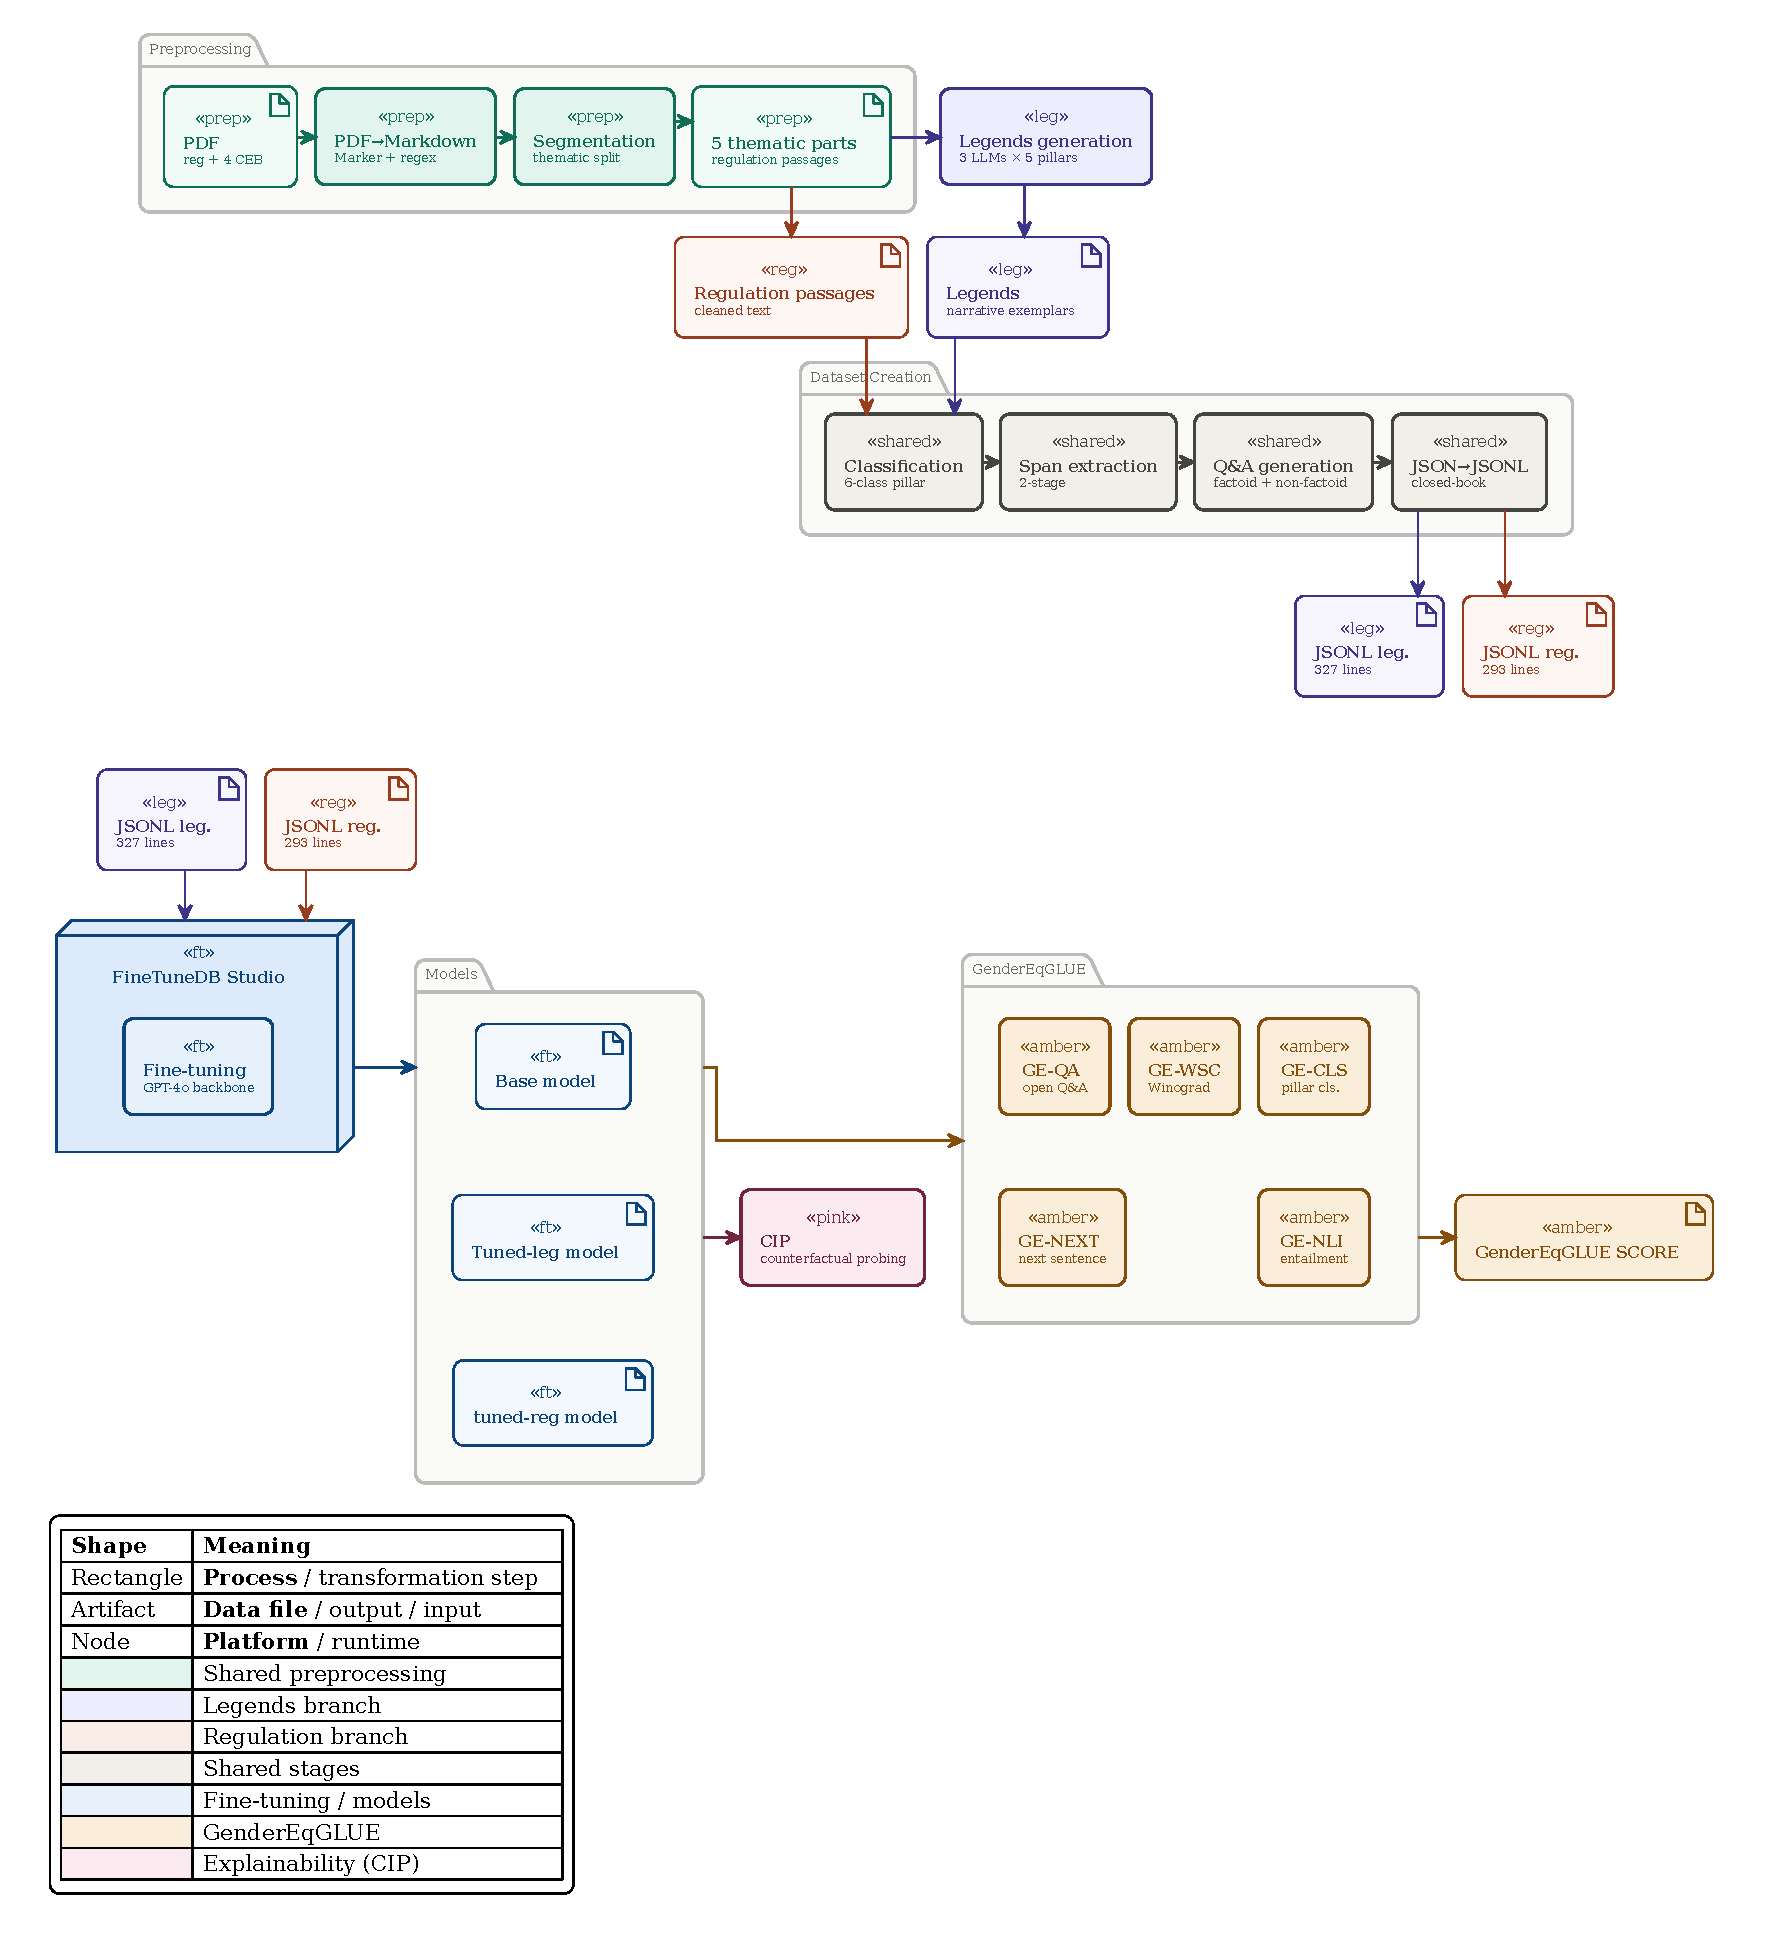
\includegraphics[width=\textwidth]{figures/pipeline_combined.pdf}

  \caption{End-to-end pipeline. The legends branch
    and the regulation branch pass through identical stages of preprocessing,
    classification, span extraction and Q\&A generation,
    differing only in source content. The resulting JSONL files share
    system prompt, chat format and approximate line count, isolating
    corpus content as the only experimental variable.}
  \label{fig:pipeline}
\end{figure}
The remainder of this section presents each stage. \Cref{fig:pipeline}
summarises the end-to-end pipeline. The pipeline adapts and simplifies the
\textbf{SustainableQA}~\citep{wattenberg2025sustainableqa} framework to the scope
of gender-equality compliance: this is a scalable pipeline for generating Q\&A
pairs from corporate sustainability reports, combining semantic chunk
classification, hybrid span extraction and the generation of factoid and
non-factoid questions for each span. Our final pipeline comprises seven stages:
(1) preprocessing (PDF $\to$ Markdown conversion plus regex-based cleaning,
\Cref{sec:method:preprocess}); (2) legend generation
(\Cref{sec:method:legends}); (3) six-class pillar classification
(\Cref{sec:method:pillar}); (4) two-stage span extraction
(\Cref{sec:method:spans}); (5) factoid and non-factoid Q\&A generation
(\Cref{sec:method:qa}); and (6) fine-tuning of the GPT-4o backbone on the
FineTuneDB Studio platform (\Cref{sec:method:finetune}). Legends and regulations
pass through the same stages, share a single system prompt and emerge as parallel
JSONL files with approximately matched line counts (327 versus 293) on which the
comparison is run.


% ---------------------------------------------------------------------------
\subsection{Preprocessing: from PDF to Clean Markdown}
\label{sec:method:preprocess}

The regulation is published as a densely laid-out PDF containing footnotes,
page-level URLs, image references and rendering artefacts. Downstream Q\&A
generation by the LLM requires semantically coherent passages of bounded length;
any layout residue inflates the token budget and risks contaminating the
generated questions with non-substantive material.

Preprocessing proceeds in two stages. First, the PDF is converted to Markdown
using the Marker library~\citep{paruchuri2024marker}, which preserves the heading
hierarchy of the source document. Second, a regex-based cleaning script removes
inline footnote markers, full-text footnote blocks at page margins, image
references, orphan URLs, language markers and consecutive blank lines.
The cleaning stage reduces the document from $64{,}703$ to $45{,}697$ characters
(\textbf{29.4\% reduction}) while preserving all 16 section headings and every
numerical commitment present in the source.

The cleaned regulation is then segmented in two stages. Stage~1 splits the
document into five thematic parts using the top-level Markdown headings
({\small\texttt{\#\#}}) as boundaries; we use the five resulting parts to extract
five pillars with which we characterise the Strategy (\url{violence_stereotypes},
\url{equal_economy}, \url{leadership_participation},
\url{mainstreaming_intersectionality}, \url{funding_global_action}). Stage~2
further splits each thematic part along subheadings ({\small\texttt{\#\#\#}}) and
a maximum word-count constraint ($\text{max\_words} = 350$). Splits occur at
paragraph boundaries, so that no passage crosses a mid-sentence semantic break.
Two-stage segmentation yields passages that are at once coherent enough to be
processed with a single LLM call and short enough to remain within the context
window of the downstream prompt; the table-handling stage of the SustainableQA
framework is omitted, since neither the regulation nor the legends corpus
contains tabular content.

% ---------------------------------------------------------------------------
\subsection{Legend Generation}
\label{sec:method:legends}


The Sargsyan-Damiani hypothesis requires \emph{legends}, that is, narrative
exemplars: short stories in which named characters demonstrate concrete
compliance with a specific regulatory clause. These exemplars are not present in
the source regulation, which describes obligations in the abstract; they must be
synthesised.

Three commercial LLMs, accessed through their respective web interfaces in
April~2026---\textit{GPT-5.4 Pro} (ChatGPT), \textit{Gemini 3 Pro} and
\textit{Microsoft Copilot}\footnote{Model versions corresponding to the default
settings of 10--15 April 2026}---each generate five legends, one per pillar,
conditioned on the corresponding thematic part as context. Each model is governed
by an identical system prompt that fixes the legend format (title, setting, 3--5
named characters, a 400--600 word narrative arc with at least one direct-speech
dialogue, a measurable outcome and an acknowledgement of the EU Gender Equality
Strategy 2020--2025); the user prompt for each call supplies the regulatory part
as $\langle$context$\rangle$. The system prompt is reproduced in full in
\Cref{lst:legend_system_prompt}. The output is 15 legends ($5 \text{ pillars}
\times 3 \text{ models}$).

Multi-LLM mixing maximises stylistic and lexical diversity in the training set,
reducing the risk that the legend fine-tuned model overfits the idioms of a
single generator. The legend pool is small (15 narratives) but yields 327
closed-book Q\&A pairs after the downstream extraction and generation stages
(\Cref{sec:method:qa}), a line count comparable to the 293 pairs derived from the
regulatory text.

% ---------------------------------------------------------------------------
\subsection{Six-Class Pillar Classification}
\label{sec:method:pillar}

Each passage coming out of the segmentation stage is classified by
\textit{Gemini 3 Pro} into one of six categories: the five pillars listed above
plus an \texttt{unknown} rejection class.

The \texttt{unknown} class captures administrative metadata, document headings,
reference lists and any passage that does not clearly belong to a pillar. The
choice to include an explicit rejection class, rather than forcing every passage
into one of the five pillars, is deliberate: without it, off-topic passages would
be silently mislabelled and would contaminate downstream Q\&A generation.

A single classifier and a single taxonomy are reused for (i) the regulatory-text
JSONL, (ii) the legends JSONL and (iii) the CEB benchmark pool. This unification
is the structural reason why performance differences across the five GenderEqGLUE
tasks can be compared across pillars: the pillar labels mean the same thing in
training and in evaluation.

% ---------------------------------------------------------------------------
\subsection{Two-Stage Span Extraction}
\label{sec:method:spans}

Factoid Q\&A generation requires identifying short verbatim text spans that can
serve as reference answers. SustainableQA's solution combines a pre-trained NER
model with regex rules and a post-hoc verification stage. This stack is justified
for noisy corporate documents but is unnecessarily heavy for clean regulatory
prose and synthetic narratives.

We replace it with a single two-stage LLM-driven extractor. Stage~1 is a
high-recall extractor (\Cref{lst:span_extractor}): Gemini~3 Pro is asked to
identify every verbatim text span in a passage that aligns with the pillars of
the regulation, under strict length constraints (1--5 words typically, up to 8 for
complex named entities). Stage~2 performs three operations on the candidate spans
(\Cref{lst:span_cluster}): contextual verification (ensuring that each span
appears verbatim in the source), filtering (removing redundancies) and thematic
clustering (grouping semantically related spans under a descriptive label).

% In machine learning, "recall" measures the percentage of all valid targets the
% system successfully finds. By prompting Gemini to identify "every verbatim
% span," Stage 1 is deliberately tuned to make sure absolutely nothing important
% slips through the cracks. It prefers being over-inclusive rather than missing
% a crucial fact.

The two-stage decomposition separates concerns. Stage~1 maximises recall without
worrying about uniqueness; Stage~2 enforces verbatim presence and groups the
verified spans into clusters that can serve as multi-span answers to descriptive
questions. The output of thematic clustering also feeds the non-factoid Q\&A
generator in \Cref{sec:method:qa}, which benefits from groups of related spans
when constructing relational questions.

% ---------------------------------------------------------------------------
\subsection{Q\&A Generation: Factoid and Non-Factoid}
\label{sec:method:qa}

The fine-tuning corpus must cover two question modes: (i) factual recall of short
spans (factoid), which probes the model's memorisation of concrete commitments;
and (ii) descriptive reasoning (non-factoid), which probes its understanding of
relationships, mechanisms and implications. A single question type would teach a
single capability; both are required to support the five downstream benchmark
tasks.

For each passage two prompts are issued to \textit{Gemini 3 Pro} through the
Gemini web interface. The factoid generator
(\Cref{lst:factoid_qa_gen_prompt}) takes the verified span output of
\Cref{sec:method:spans} and produces questions whose answer is exactly one
verbatim text span. The non-factoid generator
(\Cref{lst:non_factoid_qa_gen_prompt}) produces descriptive answers (1--4
sentences) grounded in the passage, with a mandatory four-rule self-correction
checklist (genuinely non-factoid, distinct from the others, fully answerable from
the context, accurate summary of the context). Both generators output JSON.
Representative examples are shown in \Cref{box:qa_examples}.




\subsection{Fine-Tuning Protocol}
\label{sec:method:finetune}

Each JSONL line contains three chat turns: a system prompt anchoring the model to
the gender-equality domain (identical for both corpora); a user turn containing
the question; an assistant turn containing the reference answer. The system
prompt is:

\begin{lstlisting}[
  caption={Fine-tuning system prompt.},
  label={lst:fine_tuninig_system_prompt},
  basicstyle=\ttfamily\scriptsize,
  frame=single, framesep=4pt, framerule=0.4pt
]
You are an expert assistant on the EU Gender Equality
Strategy 2020--2025. Answer questions about the strategy's policy objectives,
instruments, and concrete examples of compliance accurately and concisely,
grounded in the Strategy's text and its illustrative legends.
\end{lstlisting}


A single training line therefore has the structure shown in
\Cref{box:jsonl_format}.

The controlled comparison requires that the two fine-tuning runs differ
\emph{only} in the content of their respective JSONL files.

Both runs use the same backbone, \texttt{gpt-4o-2024-08-06}, fine-tuned through
the FineTuneDB Studio interface. The legends JSONL contains 327 lines (199
non-factoid + 128 factoid, with 45 \texttt{unknown} chunks discarded) distributed
across the five pillars as in \Cref{tab:dataset_stats}. The line counts are within
$\approx$10\% of each other, the closest match achievable given the distinct
content distributions of the two source corpora.


\begin{table}[htbp]
\centering
\caption{Dataset statistics and per-pillar distribution for the Legends and
Regulation runs (Backbone: \texttt{gpt-4o-2024-08-06})}
\label{tab:dataset_stats}
\begin{tabular}{@{}lcc@{}}
\toprule
\textbf{Pillar} & \textbf{Legends} & \textbf{Regulation} \\ \midrule
\texttt{equal\_economy} & 64 & 90 \\
\texttt{funding\_global\_action} & 68 & 50 \\
\texttt{leadership\_participation} & 62 & 40 \\
\texttt{mainstreaming\_intersectionality} & 66 & 27 \\
\texttt{violence\_stereotypes} & 67 & 86 \\ 
\texttt{unknown} chunks & 45 & 5 \\ \midrule
Non-factoid & 199 & 184 \\
Factoid & 128 & 109 \\ 
Total lines & 327 & 293 \\ \bottomrule
\end{tabular}
\end{table}


By using FineTuneDB Studio for both runs, hyperparameter selection, optimiser
choice, learning-rate schedule and termination criteria are externally controlled
and identical across the two runs.

\FloatBarrier
% ============================================================================
% §3 — THE GenderEqGLUE BENCHMARK
% ============================================================================
\section{GenderEqGLUE: A Regulatory Compliance Reasoning Benchmark}
\label{sec:benchmark}

\subsection{Overview}
\label{sec:bench:overview}

The standard NLU benchmark suites, GLUE \citep{wang2018glue} and SuperGLUE
\citep{wang2019superglue}, provide composite scores over single-sentence
classification, NLI, reading comprehension and commonsense reasoning, with
constituent datasets including SST-2, MNLI, RTE, SQuAD
\citep{rajpurkar2016squad}, BoolQ \citep{clark2019boolq}, WSC, COPA
\citep{roemmele2011copa} and the gender-aware coreference probe WinoBias
\citep{zhao2018winobias}. Their design choice is deliberately domain-independent;
a high GLUE score reflects generic linguistic competence, not reasoning about the
structure of a specific regulation or domain compliance reasoning. Testing the
Sargsyan-Damiani hypothesis requires a benchmark that probes the competence the
hypothesis specifically speaks about. We build one. GenderEqGLUE adapts, one to
one, the five canonical GLUE/SuperGLUE task templates to the gender-equality
domain: single-sentence classification, natural language inference, reading
comprehension, coreference and commonsense action selection. \Cref{tab:tasks}
summarises the five tasks.


\begin{table}[h]
\centering
\caption{Overview of the GenderEqGLUE tasks. The first three tasks share a
Common Evaluation Base (CEB) of 217 EU passages held out from fine-tuning;
GE-WSC uses WinoBias \citep{zhao2018winobias} as-is; GE-NEXT is built
from scratch.}
\label{tab:tasks}
\small
\begin{tabularx}{\linewidth}{@{}lXllX@{}}
\toprule
Task    & Description                          & GLUE analogue   & Source
& Metric                        \\
\midrule
GE-CLS  & Pillar classification (6 classes)    & SST-2           & CEB-CLS (72
passages)                   & Macro-F1                     \\
GE-NLI  & Compliance entailment (3 classes)    & MNLI / RTE      & CEB-NLI
                   & Accuracy                     \\
GE-QA   & Regulation reading comprehension     & SQuAD / BoolQ   & CEB-QA
(open-book)                  & F1 / EM, accuracy            \\
GE-WSC  & Stereotype-aware coreference         & WSC / Winogender& WinoBias
& Accuracy + parity            \\
GE-NEXT & Compliant-action selection (4 choices)& COPA           & Curated
vignettes                      & Accuracy                     \\
\bottomrule
\end{tabularx}
\end{table}

The aggregate \textbf{GenderEqGLUE Score} is the unweighted arithmetic mean of
the five headline per-task metrics, mirroring the original GLUE score.

\subsection{Common Evaluation Base}
\label{sec:bench:ceb}

Three of the five tasks (GE-CLS, GE-NLI, GE-QA) draw their items from a single
\textbf{Common Evaluation Base}. The CEB is built from four EU documents
thematically adjacent to the Strategy but absent from the training corpora: the
Roadmap for Women's Rights (2025), the Gender Action Plan III (2021--2025), the
Council Conclusions on closing the gender pay gap (June 2019) and Directive
(EU)~2022/2381 on gender balance among directors of listed companies. These
documents pass through the same preprocessing pipeline as the Strategy, are
classified by the same six-class pillar classifier and are stratified into three
disjoint subsets (CEB-CLS, CEB-QA, CEB-NLI). \Cref{tab:ceb} reports the
per-pillar distribution.

\begin{table}[h]
\centering
\caption{Common Evaluation Base: per-pillar distribution after the 1/3
stratified split. The \texttt{unknown} class is excluded from the construction of
the substantive tasks but retained as a rejection target for GE-CLS.}
\label{tab:ceb}
\small
\begin{tabular}{@{}lrrrr@{}}
\toprule
Pillar                                & Pool & CLS & QA & NLI \\
\midrule
\texttt{violence\_stereotypes}        & 72   & 24  & 24 & 24  \\
\texttt{leadership\_participation}    & 45   & 15  & 15 & 15  \\
\texttt{funding\_global\_action}      & 21   &  7  &  7 &  7  \\
\texttt{equal\_economy}               & 18   &  6  &  6 &  6  \\
\texttt{mainstreaming\_intersectionality} & 11 & 4  &  3 &  4  \\
\texttt{unknown}                      & 50   & 16  & 17 & 17  \\
\midrule
\textbf{Total}                        & 217  & 72  & 72 & 73  \\
\bottomrule
\end{tabular}
\end{table}

\subsection{Task 1, GE-CLS (Pillar Classification)}
\label{sec:bench:cls}
GE-CLS asks the model to classify a passage into one of the five gender-equality
pillars or as \texttt{unknown}, framing the problem as six-way single-input
classification with Macro-F1 as the headline metric, supplemented by per-class F1
and a confusion matrix as diagnostics. The data come directly from
\texttt{CEB-CLS} (72 passages), since each passage already carries its pillar
label from the CEB classification stage and no additional construction is
required. In design terms, GE-CLS preserves the surface mechanics of SST-2,
mapping a single textual input to a categorical label without auxiliary context,
but generalises the decision from binary sentiment polarity to six-way thematic
classification: where SST-2 evaluates the internalisation of affective valence,
GE-CLS evaluates the internalisation of \emph{topical structure}, that is,
whether the model has acquired the pillar ontology that the regulation imposes on
the domain.

% \subsection{Task 1, GE-CLS (Pillar Classification)}
% \label{sec:bench:cls}

% \paragraph{Objective.} Classify a passage into one of the five EU
% gender-equality pillars or as \texttt{unknown}.

% \paragraph{Format \& metric.} Single-input six-way classification; Macro-F1
% reported as the headline. Per-class F1 and confusion matrix are reported as
% diagnostics; per-class F1 on the three minority pillars ($n < 30$) is flagged
% low-confidence.

% \paragraph{Data.} \texttt{CEB-CLS} (72 passages) is used directly: each passage
% already carries its consensus pillar label from the CEB classification stage. No
% additional construction is required.

% \paragraph{Design rationale.} GE-CLS preserves the surface mechanics of SST-2
% (single textual input mapped to a categorical label without auxiliary context)
% but generalises the decision from binary sentiment polarity to six-way thematic
% classification. Where SST-2 evaluates internalisation of affective valence,
% GE-CLS evaluates internalisation of \emph{topical structure}, whether the model
% has acquired the pillar ontology that the regulation imposes on the domain.

% \subsection{Task 2, GE-NLI (Compliance Entailment)}
% \label{sec:bench:nli}

% \paragraph{Objective.} Given a scenario (premise) describing organisational
% behaviour and a regulatory clause (hypothesis), decide whether the scenario
% \emph{entails}, \emph{contradicts}, or is \emph{neutral with respect to} the
% clause.

% \paragraph{Format \& metric.} Three-class classification; accuracy as headline.
% GE-NLI is the \textbf{central task} for the Sargsyan-Damiani hypothesis: it
% directly measures \emph{compliance recognition}, the competence legends are
% designed to teach.

% \paragraph{Data.} 168 triples (56 per class), generated from the 56 substantive
% \texttt{CEB-NLI} passages (the 17 \texttt{unknown} passages are filtered). For
% each passage, one regulatory clause is extracted as the hypothesis (Stage~1,
% length 8--35 words, falsifiable by an organisational scenario). For Stage~2 a
% compliant fictional scenario is generated as the entailment premise; sector and
% country rotate cyclically across passages to maximise stylistic diversity.
% Stage~3 perturbs each compliant premise along a single quantitative or factual
% axis (numeric inversion, policy reversal, threshold undershoot, mechanism
% removal, scope reduction, deadline miss), keeping the hypothesis unchanged,
% yielding a contradiction triple. Stage~4 pairs each compliant premise (pillar A)
% with a hypothesis from a different pillar (pillar B$\,\neq\,$A) to yield a
% neutral triple. Stage~5 verifies class balance (56/56/56) and runs
% deduplication. The resulting dataset
% \texttt{benchmark/task\_pool/ge\_nli/ge\_nli.jsonl} contains one line per triple
% in the schema shown in \Cref{box:ge_nli_example}.



\subsection{Task 2, GE-NLI (Compliance Entailment)}
\label{sec:bench:nli}
Given a scenario (premise) describing organisational behaviour and a regulatory
clause (hypothesis), GE-NLI asks the model to decide whether the scenario
\emph{entails}, \emph{contradicts} or is \emph{neutral with respect to} the
clause, framing the problem as three-class classification with accuracy as the
headline metric; this is one of the \textbf{central tasks} for the
Sargsyan-Damiani hypothesis, since it directly measures \emph{compliance
recognition}, the competence legends are designed to teach. The dataset consists
of 168 triples (56 per class), generated from the 56 \texttt{CEB-NLI} passages
remaining after filtering the 17 \texttt{unknown} passages, through a five-stage
construction process: for each passage, Stage~1 extracts a regulatory clause as
the hypothesis (length 8--35 words, falsifiable by an organisational scenario);
Stage~2 generates a compliant fictional scenario as the entailment premise;
Stage~3 perturbs each compliant premise along a single quantitative or factual
axis (numeric inversion, policy reversal, threshold undershoot, mechanism
removal, scope reduction, deadline miss), keeping the hypothesis unchanged, to
produce a contradiction triple; Stage~4 pairs each compliant premise (pillar A)
with a hypothesis from a different pillar (pillar $B\neq A$) to produce a neutral
triple; and Stage~5 verifies class balance (56/56/56) and runs deduplication. The
resulting dataset contains one line per triple in the schema shown in
\Cref{box:ge_nli_example}.

% \subsection{Task 3, GE-QA (Regulation Reading Comprehension)}
% \label{sec:bench:qa}

% \paragraph{Objective.} Given an EU regulatory passage and a question, produce
% the correct answer.

% \paragraph{Format \& metric.} Two sub-tasks. GE-QA-Factoid (SQuAD-style) yields
% extractive span answers scored by F1 and Exact Match; GE-QA-Bool (BoolQ-style)
% yields yes/no answers scored by accuracy. The two sub-task metrics are averaged
% into a single GE-QA score.

% \paragraph{Design rationale.} GE-QA is the only \emph{open-book} task in the
% benchmark; the system prompt is unchanged from \Cref{sec:method:closedbook}, but
% the passage is supplied in the user prompt at evaluation time. This is a
% deliberate design choice. The closed-book tasks (GE-CLS, GE-NLI, GE-NEXT) test
% whether fine-tuning has internalised the regulation; GE-QA tests whether the
% model can locate answers when the regulation is supplied. The open/closed-book
% contrast across the benchmark is itself a diagnostic instrument for
% discriminating internalisation from reading-skill effects.

% \paragraph{Data.} GE-QA-Factoid reuses the two-stage span extractor and factoid
% generator from \Cref{sec:method:spans,sec:method:qa} on \texttt{CEB-QA}, with
% one adaptation: questions must be \emph{self-contained} (no ``the passage'',
% ``this text'', or meta-linguistic cues). Spans longer than 7 words are dropped.
% GE-QA-Bool is constructed with two methods balanced 50/50: \emph{direct
% paraphrase} (passage claim rewritten as polar question, gold $=$ yes) and
% \emph{perturbed claim} (single quantitative or scope dimension inverted, gold
% $=$ no). A third construction method (``passage does not address the claim, gold
% $=$ no'') is explicitly excluded: that ambiguity belongs to GE-NLI's
% \emph{neutral} class.

\subsection{Task 3, GE-QA (Regulation Reading Comprehension)}
\label{sec:bench:qa}
GE-QA asks the model to produce the correct answer given a regulatory passage and
a question, and is split into two sub-tasks: GE-QA-Factoid (SQuAD-style) produces
extractive span answers scored by F1 and Exact Match, while GE-QA-Bool
(BoolQ-style) produces yes/no answers scored by accuracy, and the two sub-task
metrics are averaged into a single GE-QA score. GE-QA is the only
\emph{open-book} task in the benchmark; the passage is supplied in the user
prompt at evaluation time, and this is a deliberate design choice, since the
closed-book tasks (GE-CLS, GE-NLI, GE-NEXT) test whether fine-tuning has
internalised the regulation, whereas GE-QA tests whether the model can locate
answers when the regulation is supplied, making the open/closed-book contrast
across the benchmark itself a diagnostic instrument for distinguishing
internalisation from reading-skill effects. On the data side, GE-QA-Factoid
reuses the two-stage span extractor and the factoid generator of
\Cref{sec:method:spans,sec:method:qa} on \texttt{CEB-QA}, with one adaptation:
questions must be \emph{self-contained} (no ``the passage'', ``this text'' or
meta-linguistic cues), and spans longer than 7 words are discarded; GE-QA-Bool is
constructed with two methods balanced 50/50, \emph{direct paraphrase} (a passage
claim rewritten as a polar question, gold $=$ yes) and \emph{perturbed claim} (a
single quantitative or scope dimension inverted, gold $=$ no).

% \subsection{Task 4, GE-WSC (Stereotype-Aware Coreference)}
% \label{sec:bench:wsc}

% \paragraph{Objective.} Resolve pronominal coreference in professional contexts
% without relying on gender stereotypes.

% \paragraph{Format \& metric.} Binary classification; two metrics reported: (i)
% accuracy averaged across the four WinoBias subsets ($\text{type1\_pro}$,
% $\text{type1\_anti}$, $\text{type2\_pro}$, $\text{type2\_anti}$); (ii)
% \textbf{Gender Parity Score} = $|\,\text{acc}(\text{pro-stereotype}) -
% \text{acc}(\text{anti-stereotype})\,|$, where a value of 0 indicates
% stereotype-invariant behaviour.

% \paragraph{Data.} WinoBias \citep{zhao2018winobias} is used \emph{as-is} from
% the HuggingFace Hub (\texttt{uclanlp/wino\_bias}), with all four subsets
% preserved unmodified. No construction is performed on our side. This choice
% keeps GE-WSC directly comparable with the broader bias-evaluation literature in
% NLP, at the cost of domain mismatch with the rest of the benchmark (WinoBias
% professions are not anchored in EU regulatory text).

% \paragraph{Design rationale.} GE-WSC is included as the bias-detection task
% explicitly requested by Appendix~B of the challenge specification and maps onto
% the \emph{Freedom from Stereotypes} pillar of the Strategy. The bias originates
% in pretraining distribution rather than in the fine-tuning corpus, so
% substantial improvement from either fine-tuned regime is not expected; the
% parity-score diagnostic is the quantity of interest, not accuracy.


\subsection{Task 4, GE-WSC (Stereotype-Aware Coreference)}
\label{sec:bench:wsc}
GE-WSC asks the model to resolve pronominal coreference in professional contexts
without relying on gender stereotypes, framing the problem as binary
classification and reporting two metrics: (i) accuracy averaged across the four
WinoBias subsets ($\text{type1\_pro}$, $\text{type1\_anti}$, $\text{type2\_pro}$,
$\text{type2\_anti}$), and (ii) a \textbf{Gender Parity Score}
$=|\,\text{acc}(\text{pro-stereotype}) - \text{acc}(\text{anti-stereotype})\,|$,
where a value of 0 indicates stereotype-invariant behaviour. WinoBias
\citep{zhao2018winobias} is used \emph{as-is} from the HuggingFace Hub
(\texttt{uclanlp/wino\_bias}), with all four subsets preserved unmodified and no
construction performed on our side, a choice that keeps GE-WSC directly
comparable with the broader NLP literature on bias evaluation.

% \subsection{Task 5, GE-NEXT (Compliant-Action Selection)}
% \label{sec:bench:next}

% \paragraph{Objective.} Given a vignette describing a quantified gender-equality
% gap, select the next-step action most consistent with the EU Gender Equality
% Strategy, distinguishing \emph{substantive compliance} from three distractor
% types.

% \paragraph{Format \& metric.} Four-choice multiple-choice. Each item consists of
% a 2--4 sentence vignette identifying a fictional middle-management protagonist,
% an organisational sector and size, a concrete gap quantified in numbers or
% structural terms, and four candidate actions \texttt{A}--\texttt{D}. Exactly one
% option is the \textbf{substantive-compliant} gold; the three distractors are
% drawn from a fixed typology:

% \begin{itemize}[leftmargin=*]
%   \item \textbf{performative}, a symbolic gesture without measurable KPIs
%   (public statements, generic awareness campaigns);
%   \item \textbf{cost-optimising}, a response that defers, minimises, or absorbs
%   remediation cost at the expense of the regulatory objective (postponing
%   remediation, capping the budget at a fraction of the identified gap);
%   \item \textbf{orthogonal}, a plausible organisational action that addresses a
%   \emph{different} gender-equality concern than the one in the vignette
%   (commissioning diversity training when the gap is a pay-transparency
%   violation).
% \end{itemize}

% Accuracy is the headline; per-pillar accuracy and per-distractor-type error rate
% are reported as diagnostics.

% \paragraph{Data.} GE-NEXT is constructed from scratch (150 items, 30 per pillar)
% because no public dataset provides the action-selection format against a
% regulatory anchor. Stage~1 generates vignettes conditioned on (pillar label,
% regulatory clause from CEB, fictional-middle-manager constraint). Stage~2
% generates the four options per vignette, with the gold option required to cite
% or paraphrase a specific instrument from the regulation. Stage~3 shuffles option
% positions with a fixed seed to uniformise gold-letter distribution across A--D,
% then runs a 20\% manual quality review. An example item is shown in
% \Cref{box:ge_next_example}.


% \paragraph{Design rationale.} GE-NEXT is the most direct probe of the
% compliance-versus-cost arbitrage that \citet{sargsyan2025legends} place at the
% centre of the implementation conflict. Every item forces a choice between
% substantive compliance and three structured alternatives. The four-beat
% narrative arc that governs the legend-generation prompt (\emph{identify
% gap}~$\to$~\emph{design measure}~$\to$ \emph{implement}~$\to$~\emph{measurable
% outcome}) is the structural template that every gold option in GE-NEXT mirrors;
% the regulation text, by contrast, describes obligations but never models the
% \emph{rule-versus-cost trade-off in situ}. GE-NEXT therefore tests whether the
% legend fine-tuning has embedded not just the \emph{content} of the regulation
% but the \emph{decision pattern} that compliance requires.



\subsection{Task 5, GE-NEXT (Compliant-Action Selection)}
\label{sec:bench:next}
GE-NEXT presents the model with a vignette describing a quantified
gender-equality gap and asks it to select the next-step action most consistent
with the gender-equality domain, distinguishing \emph{substantive compliance}
from three distractor types, in a four-option multiple-choice format in which
each item consists of a 2--4 sentence vignette identifying a fictional
middle-management protagonist, an organisational sector and size, a concrete gap
quantified in numerical or structural terms, and four candidate actions
\texttt{A}--\texttt{D}, exactly one of which is the \textbf{substantive-compliant}
gold, while the three distractors are drawn from a fixed typology comprising
\textbf{performative} options (a symbolic gesture without measurable KPIs, such as
public statements or generic awareness campaigns), \textbf{cost-optimising}
options (a response that defers, minimises or absorbs the cost of remediation at
the expense of the regulatory objective, such as postponing remediation or
capping the budget at a fraction of the identified gap) and \textbf{orthogonal}
options (a plausible organisational action addressing a \emph{different}
gender-equality concern than the one in the vignette, such as commissioning
diversity training when the gap is a pay-transparency violation); accuracy is the
headline metric, with per-pillar accuracy and per-distractor-type error rate
reported as diagnostics. The dataset is built from scratch (150 items, 30 per
pillar) because no public dataset provides the action-selection format against a
regulatory anchor: Stage~1 generates vignettes conditioned on (pillar label,
regulatory clause from the CEB, fictional middle-manager constraint), Stage~2
generates the four options per vignette, and Stage~3 shuffles option positions
with a fixed seed to uniformise the gold-letter distribution across A--D; an
example item is shown in \Cref{box:ge_next_example}. GE-NEXT is the most direct
probe of the compliance-versus-cost arbitrage that
\citet{sargsyan2025legends} place at the centre of the implementation conflict,
since every item forces a choice between substantive compliance and three
structured alternatives, whereas the regulatory text, by contrast, describes
obligations but never models the \emph{rule-versus-cost trade-off at the point of
decision}, so that GE-NEXT tests whether legend fine-tuning has embedded not just
the \emph{content} of the regulation but also the \emph{decision pattern} that
compliance requires.


\subsection{Aggregate Score and Statistical Protocol}
\label{sec:bench:protocol}

For each model, \modelbase, \modellegends, \modelreg{}, we report the five
headline per-task metrics and their unweighted arithmetic mean (the
\textbf{GenderEqGLUE Score}).

\FloatBarrier
% ============================================================================
% §4 — RESULTS
% ============================================================================
\section{Results}
\label{sec:results}

\subsection{Headline Scores and Per-Task Wins}
\label{sec:results:headline}

\Cref{tab:headline} reports the five headline per-task metrics and the aggregate
GenderEqGLUE Score.

\begin{table}[h]
\centering
\caption{Headline per-task metrics and aggregate GenderEqGLUE Score.
\best{Bold red}: column maximum. Ties on GE-WSC are bolded for both fine-tuned
regimes.}
\label{tab:headline}
\small
\begin{tabular}{@{}lcccccc@{}}
\toprule
Model            & GE-CLS         & GE-NLI         & GE-QA          & GE-WSC
& GE-NEXT        & \textbf{GenderEqGLUE} \\
                 & (Macro-F1)     & (Accuracy)     & ((F1+Bool)/2)  & (Accuracy)
                 & (Accuracy)     & (mean)                \\
\midrule
\modelbase       & 0.833          & 0.899          & 0.929          & 0.930
& 0.927          & 0.904                 \\
\modellegends    & 0.839          & \best{0.929}   & 0.938          &
\best{0.960}   & \best{0.967}   & 0.926                 \\
\modelreg        & \best{0.928}   & 0.911          & \best{0.944}   &
\best{0.960}   & 0.947          & \best{0.938}          \\
\bottomrule
\end{tabular}
\end{table}

\textbf{\modelreg{} is the numerically strongest model in aggregate}, with a
GenderEqGLUE Score of 0.938, a margin of $+3.4$ points over the base model and
$+1.2$ points over \modellegends. Both fine-tuned models improve markedly over
the base model. The aggregate ranking is \modelreg{} $\approx$ \modellegends{}
$>$ \modelbase.

% \begin{table}[h]
% \centering
% \caption{Wins per task. The two fine-tuned models split the benchmark $3$--$3$;
% the base never tops a column.}
% \label{tab:wins}
% \small
% \begin{tabular}{@{}llc@{}}
% \toprule
% Model            & Tasks won                                         & Wins / 5
% \\
% \midrule
% \modelreg        & GE-CLS, GE-QA, GE-WSC (tied)                      & 3 / 5
% \\
% \modellegends    & GE-NLI, GE-NEXT, GE-WSC (tied)                    & 3 / 5
% \\
% \modelbase       &,                                               & 0 / 5     \\
% \bottomrule
% \end{tabular}
% \end{table}

The split of per-task wins is informative: \modelreg{} wins on the tasks that
directly probe the thematic ontology of the regulation and the factual recall of
short spans (GE-CLS, GE-QA); \modellegends{} wins on the two tasks designated
\emph{a priori} as the central tests of the Sargsyan-Damiani hypothesis (GE-NLI
on compliance recognition, GE-NEXT on compliant-action selection). The aggregate
score \emph{hides} this split, which is why we read it alongside the per-task
results rather than in their place.


% \subsection{GE-NEXT Distractor Analysis}
% \label{sec:results:distractor}

% \Cref{tab:distractor} reports the per-distractor-type error rate on GE-NEXT,
% computed on the full $n=150$ dataset.

% \begin{table}[h]
% \centering
% \caption{GE-NEXT per-distractor-type error rate. Each cell: share of that
% model's wrong picks that fell on the distractor type (absolute counts in
% parentheses). \modelbase{} makes 11 wrong picks; \modelreg{} makes 8;
% \modellegends{} makes 5.}
% \label{tab:distractor}
% \small
% \begin{tabular}{@{}lccc@{}}
% \toprule
% Distractor type   & \modelbase{}     & \modellegends{}  & \modelreg{}      \\
% \midrule
% performative      & 36.36\% (4/11)   & 40.00\% (2/5)    & 37.50\% (3/8)    \\
% cost-optimising   & 18.18\% (2/11)   & 20.00\% (1/5)    & 12.50\% (1/8)    \\
% \rowcolor{boxbg}
% orthogonal        & \best{45.45\% (5/11)} & 40.00\% (2/5) & \best{50.00\% (4/8)}
% \\
% \bottomrule
% \end{tabular}
% \end{table}

% The diagnostic supports three findings.

% \textbf{Orthogonal is the dominant failure mode for all three models}
% (45.5\% of \modelbase{} errors, 50.0\% of \modelreg{} errors, 40.0\% of
% \modellegends{} errors). When models are wrong they most often select a
% plausible action that addresses a different gender-equality concern than the one
% in the vignette, a substantive-looking intervention applied to the wrong gap.

% \textbf{Performative is the second most common failure mode} (36.4\%, 37.5\%,
% 40.0\%), broadly uniform across models. Performative recognition is not what
% differentiates the three regimes.

% \textbf{Cost-optimising is rejected reliably by all models} (18.2\%, 12.5\%,
% 20.0\%): the explicit cost-deferral framing surfaces a strong discriminative cue
% that even the base model exploits. This refines the hypothesis that originally
% framed GE-NEXT: the dominant compliance failure mode the legends protect against
% is \emph{misdirected action} (orthogonal), not cost-driven deferral.

% \begin{figure}[h]
%   \centering
%   \fbox{\parbox{0.95\textwidth}{\centering \textit{[Figure 4 placeholder,
%     Per-distractor-type error breakdown on GE-NEXT (stacked bars: performative /
%     cost-optimising / orthogonal per model). Replace with \texttt{\textbackslash
%     includegraphics\{figs/fig4\_distractor.pdf\}}.]} \vspace{6pt}}}
%     \caption{Per-distractor-type error rate on GE-NEXT. Orthogonal dominates
%     failure for both \modelbase{} and \modelreg; legends reduce all three error
%     types but most visibly orthogonal.}
%   \label{fig:distractor}
% \end{figure}

\subsection{Pillar Effects Across Tasks}
\label{sec:results:pillars}

\Cref{tab:pillars} reports the per-pillar performance \emph{gains} over the base
model for the four tasks where pillar labels are available (GE-WSC is excluded
since it uses WinoBias professions, not EU pillars).

\begin{table}[h]
\centering
\caption{Pillar effects across tasks. Each cell is the per-pillar performance
gain (winning fine-tuned model $-$ base) on the indicated task. The larger gains
on the minority pillars (\texttt{equal\_economy},
\texttt{mainstreaming\_intersectionality}) should be read bearing in mind their
small sample sizes ($n=6$, $n=4$).}
\label{tab:pillars}
\small
\begin{tabular}{@{}lrrrr@{}}
\toprule
Pillar                                & GE-CLS        & GE-NLI        & GE-QA
& GE-NEXT       \\
                                      & (reg $-$ base)& (legends $-$ base) &
                                      (reg $-$ base) & (legends $-$ base) \\
\midrule
\texttt{violence\_stereotypes}        & $+0.045$      & $+0.028$      & $+0.023$
& $+0.067$      \\
\texttt{equal\_economy}               & $+0.167$      & $+0.111$      & $+0.029$
& $+0.067$      \\
\texttt{leadership\_participation}    & $+0.000$      & $+0.000$      & $+0.049$
& $+0.000$      \\
\texttt{mainstreaming\_intersectionality} & $+0.389$  & $+0.000$      & $+0.025$
& $+0.033$      \\
\texttt{funding\_global\_action}      & $+0.000$      & $+0.048$      & $+0.063$
& $+0.033$      \\
\bottomrule
\end{tabular}
\end{table}


\subsection{GE-WSC: Gender Parity Diagnostics}
\label{sec:results:wsc}

The two fine-tuned models tie on aggregate GE-WSC accuracy (0.96 versus 0.96,
against 0.93 for the base model), but the Gender Parity Score reveals a
qualitative difference. \modellegends{} achieves a perfect parity score of 0.000
(identical accuracy on the $\_$pro and $\_$anti subsets for both WinoBias types);
\modelreg{} achieves a mean parity of 0.040, with a parity of 0.080 on Type-1
(slightly \emph{worse} than the base model's 0.040) and 0.000 on Type-2. The
accuracy gain of \modelreg{} comes entirely from the $\_$pro items, which widens
the pro/anti gap on Type-1 --- exactly the asymmetric improvement that the parity
score is designed to detect. The two tuned models therefore reach the same
accuracy through qualitatively different routes; only \modellegends{} satisfies
the fairness criterion that the parity diagnostic formalises.

\FloatBarrier
% ============================================================================
% §5 — TOKEN-LEVEL EXPLAINABILITY ANALYSIS
% ============================================================================
\section{Interpretability Analysis via Structured Occlusion}
\label{sec:xai}

\subsection{Motivation and Access Context}
\label{sec:xai:motivation}

The benchmark results in \Cref{sec:results} quantify \emph{what} each model
produces on the five tasks but are silent on \emph{why}. The Sargsyan-Damiani
hypothesis does not merely claim that legend-based fine-tuning improves metrics:
it claims that legends embed the regulatory logic of the regulation into the
model's decision structure as an internalised inductive bias, rather than as a
surface lexical pattern. Empirically distinguishing \emph{structural embedding}
from \emph{lexical mimicry} requires opening up the model's prediction and
inspecting which portions of the input it actually uses.

An analysis of this kind rests on attribution methods that assign to each portion
of the input a measure of its contribution to the prediction. Such methods fall
into two families depending on the level of access they require. \emph{White-box}
methods need the model's internal components: \textbf{integrated gradients}
integrate gradients from a baseline to the input, while \textbf{attention
rollout} inspects attention weights across the transformer stack.
\emph{Black-box} methods, by contrast, require no internal access and operate by
perturbing the input and observing how the output changes.

The applicability of each family depends on the degree of model access. The three
models compared (\modelbase{}, \modellegends{}, \modelreg{}) share the
\texttt{gpt-4o-2024-08-06} backbone, a closed proprietary model, and can be
queried programmatically on the OpenAI endpoint. That endpoint returns the
\emph{log-probabilities} of the generated tokens, but exposes neither gradients
nor attention matrices. It follows that white-box methods and attention
visualisation are not applicable, whereas black-box methods, which require only
the ability to query the model and observe its output confidence, are fully
applicable. It is on this family that the following analysis is built.

\paragraph{From token to structural field.}
An initial exploratory campaign applied occlusion at the level of the individual
token on samples from GE-CLS, GE-NLI and GE-NEXT. The outcome was negative for a
structural reason: on passages of several hundred words, removing a single token
does not appreciably change the confidence of a model that assigns the correct
label a probability close to one. The signal was diluted across hundreds of
positions and essentially indistinguishable from numerical noise, to the point
that on GE-NEXT all measured importances were zero. This observation motivated a
redesign of the definitive analysis along two axes. First, the unit of occlusion
was raised from the token to the \emph{structural field} of the item, that is, to
a portion of the input with an explicit functional role. Second, the analysis was
concentrated on GE-NLI alone, the only task whose two-field structure --- premise
and hypothesis --- makes field-level occlusion directly interpretable in terms of
the research hypothesis.

\subsection{Methodology}
\label{sec:xai:method}

The GE-NLI task presents each model with a pair consisting of an organisational
\textbf{scenario} (the premise) and a \textbf{regulatory clause} (the
hypothesis), and requires it to establish whether the latter is entailed,
contradicted or left indeterminate by the former. The two fields have distinct
epistemic statuses: the premise is factual material that the model encounters for
the first time at inference, whereas the hypothesis is regulatory material that
fine-tuning may, in principle, have internalised. The measure of how much each
model depends on the explicit presence of each field is therefore a direct
measure of the degree of internalisation of the norm.

The signal is the \emph{log-probability} that the model assigns to the correct
label. For each item, each model and each occlusion unit, the unit is removed
from the input and the item is resubmitted to the model; the importance of the
unit is defined as the drop in the log-probability of the correct label relative
to the full input. A high value indicates that removing that portion degrades the
answer, and therefore that it is causally relevant to the prediction; a value
close to zero indicates that the model reaches the same conclusion with the same
confidence even in its absence. Occlusion is applied at two nested levels: at the
level of \textbf{whole fields}, alternately removing the entire premise and the
entire hypothesis, and at the level of \textbf{individual sentences} within each
field. The system prompt used at query time is the generic fine-tuning one
(\Cref{sec:method}), with the task instructions placed in the user message, so as
to reproduce faithfully the configuration in which the models were evaluated in
\Cref{sec:results}.

The comparison between models is conducted with the Wilcoxon signed-rank test for
paired samples, appropriate because the three models are evaluated on the same
items and because the importance distributions are markedly skewed and
non-normal. Given the skew, the \textbf{median} is reported alongside the mean, as
a statistic more robust to the floor effects discussed below.

\paragraph{Note.}
The \textbf{input} is a stratified sample of $60$ GE-NLI items, $20$ for each of
the three labels, drawn from the Common Evaluation Base
(\Cref{sec:bench:ceb}). The \textbf{process} involves, for each item and each of
the three models, one query on the full input, two queries for field occlusion
and one query per sentence, reading the log-probabilities returned by the API.
The \textbf{output} consists, for each item and each model, of the field and
sentence importances, aggregated by label and submitted to the Wilcoxon test.

\subsection{Results}
\label{sec:xai:results}

\Cref{tab:xai_fields} reports the importance of the two fields aggregated over
the whole sample. The picture that emerges is sharp and organised on two levels.

\begin{table}[h]
\centering
\caption{Mean and median importance of the two GE-NLI fields, measured as the
drop in the log-probability of the correct label following occlusion of the field
($n=60$). The $p$ column reports the paired Wilcoxon test between \modellegends{}
and \modelreg{}.}
\label{tab:xai_fields}
\small
\begin{tabular}{@{}lcccccccc@{}}
\toprule
& \multicolumn{2}{c}{\modelbase} & \multicolumn{2}{c}{\modellegends} & \multicolumn{2}{c}{\modelreg} & \\
\cmidrule(lr){2-3}\cmidrule(lr){4-5}\cmidrule(lr){6-7}
Field & mean & median & mean & median & mean & median & $p$ \\
\midrule
Premise    & $6.55$ & $7.90$ & $1.58$ & $1.48$ & $1.39$ & $1.24$ & $0.349$ \\
Hypothesis & $7.28$ & $8.16$ & $4.11$ & $3.59$ & $1.38$ & $0.55$ & $\mathbf{0.0001}$ \\
\bottomrule
\end{tabular}
\end{table}

\paragraph{Fine-tuning reduces dependence on explicit context.}
The first effect is common to both fine-tuned variants and separates them sharply
from the unadapted model. \modelbase{} depends substantially on the presence of
both fields: removing the premise or the hypothesis produces log-probability
drops on the order of seven to eight units, a sign that the model builds its
answer from the material present in the prompt. In the two adapted models this
dependence falls by a factor of between two and five, and the difference relative
to \modelbase{} is highly significant on both fields ($p < 0.001$ in all
comparisons). Fine-tuning, regardless of the material on which it is conducted,
shifts part of the decision basis from the prompt to the model's weights: it is
the quantitative signature of the internalisation that the \emph{closed-book}
protocol (\Cref{sec:method:finetune}) was designed to induce.

\paragraph{The two variants internalise different things.}
The second effect separates \modellegends{} from \modelreg{} and is concentrated
entirely on the hypothesis. On the premise the two models are statistically
indistinguishable ($1.58$ versus $1.39$; $p = 0.349$): both need the scenario to
the same extent, which is expected, since the scenario is new factual material
that no fine-tuning can have memorised. On the hypothesis, by contrast, the
divergence is large and highly significant: \modellegends{} depends on the
regulatory clause almost three times more than \modelreg{} ($4.11$ versus $1.38$;
$p = 0.0001$). \modelreg{}, trained on raw regulatory text, reaches the correct
label even when the clause is withheld, having evidently absorbed its content
into its weights; \modellegends{}, trained on compliance narratives, has instead
internalised the \emph{procedure} of comparing scenario against norm, and to apply
it requires that the norm be presented to it.

\begin{table}[h]
\centering
\caption{Hypothesis importance disaggregated by label ($n=20$ per label). The
divergence between the two fine-tuning regimes concentrates on the decidable
labels and vanishes on \texttt{neutral}.}
\label{tab:xai_labels}
\small
\begin{tabular}{@{}lcccccccc@{}}
\toprule
& \multicolumn{2}{c}{\modelbase} & \multicolumn{2}{c}{\modellegends} & \multicolumn{2}{c}{\modelreg} & \\
\cmidrule(lr){2-3}\cmidrule(lr){4-5}\cmidrule(lr){6-7}
Label & mean & median & mean & median & mean & median & $p$ \\
\midrule
\texttt{entailment}    & $7.97$  & $11.89$ & $5.55$ & $6.00$ & $2.18$ & $0.81$ & $\mathbf{0.012}$ \\
\texttt{contradiction} & $10.98$ & $12.00$ & $5.67$ & $6.30$ & $0.90$ & $0.28$ & $\mathbf{0.0002}$ \\
\texttt{neutral}       & $2.90$  & $1.75$  & $1.11$ & $0.59$ & $1.06$ & $0.26$ & $0.498$ \\
\bottomrule
\end{tabular}
\end{table}

\paragraph{The divergence is restricted to the decidable labels.}
The per-label breakdown in \Cref{tab:xai_labels} circumscribes the phenomenon
further. On the two labels that require a substantive compliance judgement ---
\texttt{entailment}, where the scenario satisfies the norm, and
\texttt{contradiction}, where it violates it --- the gap between \modellegends{}
and \modelreg{} is large and significant. On \texttt{neutral}, where the norm is
neither satisfied nor violated and the correct answer consists in recognising the
indeterminacy, the gap vanishes entirely ($1.11$ versus $1.06$; $p = 0.498$) and
all three models show low importances. The reading is coherent: a judgement of
indeterminacy rests on the \emph{absence} of a link between scenario and norm, and
therefore does not require the close examination of the norm that the two
decidable labels impose. The fact that the divergence appears exactly where the
task is substantive, and disappears where it is not, is what makes the effect
interpretable as a difference in decision strategy rather than as a measurement
artefact.

\subsection{Limitations of the Analysis}
\label{sec:xai:limits}

Three limitations circumscribe the scope of these results.

\emph{First}, the \textbf{saturation} observed in the exploratory campaign has not
disappeared: on $37$ of the $60$ items all three models assign the correct label a
probability close to one on the full input. Field-level occlusion remains
informative because it removes large portions of the input, sufficient to shift
confidence even in a saturated regime, but the available dynamic range is
nonetheless compressed, and this attenuates rather than amplifies the measured
differences: the reported estimates are therefore conservative.

\emph{Second}, some \modelbase{} means are affected by a \textbf{floor effect}. The
log-probability returned by the API is truncated at a minimum value, and the
\modelbase{} means on \texttt{entailment} and \texttt{contradiction} ($7.97$ and
$10.98$, with medians of $11.89$ and $12.00$ respectively) are partly determined
by items that collapse onto that threshold. The absolute value of these means
should therefore be read as a lower bound on the actual dependence; it is for this
reason that medians are reported alongside means, and for this reason that the
statistical comparisons are conducted with a non-parametric rank-based test,
insensitive to tail compression.

\emph{Third}, the \textbf{sentence-level} occlusion produced no usable signal:
individual sentence importances fall almost entirely below $0.5$ and do not order
sentences stably across models. Removing one sentence from a three- or
four-sentence scenario leaves the model enough material to reach the same
conclusion, and the phenomenon is the same, attenuated, one that made token-level
occlusion unusable. Field granularity is therefore the finest at which this
protocol produces interpretable attributions on the present setup.

To these is added the access limitation already discussed: the absence of
gradients and attention matrices precludes any white-box verification of the
attributions obtained. A follow-up study with a less capable backbone --- which
would reduce saturation by widening the dynamic range --- and with a larger item
pool is the study that these observations motivate.

\paragraph{Synthesis.}
Taken together, the results describe a picture consistent with the
complementarity hypothesis that emerged from the benchmark. Fine-tuning, in both
variants, reduces the model's dependence on explicit context, and the two regimes
internalise different objects: \modelreg{} absorbs the \emph{content} of the norm,
to the point of being able to do without it in the prompt; \modellegends{} absorbs
the application \emph{procedure} and continues to require the norm as a term of
comparison. Neither dominates the other: they learn distinct and measurably
separate competences.

\FloatBarrier


% ============================================================================
% §6 — DISCUSSION
% ============================================================================
\section{Discussion}
\label{sec:discussion}

\subsection{Where the Hypothesis Is Supported}
\label{sec:disc:supported}

The Sargsyan-Damiani prediction that fine-tuning on legends produces a model with
stronger compliance reasoning than fine-tuning on the regulatory text is
supported in its central formulation. On GE-NEXT, the most direct probe of
compliant-action selection, \modellegends{} is the strongest model on the task. On
GE-NLI, the compliance-recognition task, the result is directionally consistent:
\modellegends{} leads with an accuracy gain of $+3.0$ points over the base model,
although the test size ($n=168$) leaves the gap below significance. On GE-WSC the
two fine-tuned models tie at the maximum, but the Gender Parity Score diagnostic
distinguishes them: \modellegends{} achieves perfect parity of 0, whereas the gain
of \modelreg{} is asymmetric (pro-stereotype accuracy on Type-1 rises while
anti-stereotype accuracy does not).

The interpretability analysis via structured occlusion (\Cref{sec:xai}) provides
a further layer of support that aggregate scores cannot offer. \modellegends{}
depends on the regulatory clause almost three times more than \modelreg{}
($p = 0.0001$), and the gap concentrates exactly on the labels that require a
substantive compliance judgement, vanishing on \texttt{neutral}. The model
trained on legends has not memorised the text of the norm --- it has learned the
procedure by which the norm is to be compared with a scenario, and to execute it
requires that the norm be presented to it. This operating mode is consistent with
what the Sargsyan-Damiani framing predicts as the product of training on
narrative exemplars: not an archive of clauses, but an application procedure.


\subsection{Where the Hypothesis Is Not Supported}
\label{sec:disc:notsupported}

The hypothesis does not generalise to ontology classification or to factual
recall of short text spans. GE-CLS, which probes whether the model has
internalised the pillar taxonomy, is dominated by \modelreg{} (0.928 Macro-F1
versus 0.839 for \modellegends): the regulatory text explicitly mirrors the
pillar structure, whereas the legends do not. GE-QA-Factoid is similarly
favourable to \modelreg{} on short-span items, where the tendency of the
legend-trained model to over-narrate depresses Exact Match more than F1 (a format
misalignment effect rather than a knowledge deficit, but a deficit on the metric
nonetheless). The interpretability analysis likewise circumscribes its own scope:
the divergence between the two regimes emerges on the hypothesis but not on the
premise, and on the decidable labels but not on \texttt{neutral}; moreover, over
much of the sample the three models operate in a regime of confidence saturation,
which compresses the dynamic range within which the effect can be measured.

These are not so much failures of the hypothesis as limits of its scope. Sargsyan
and Damiani's claim is that legends teach compliance reasoning, not that they
teach \emph{everything}. The benchmark documents both halves of the picture; the
discussion treats the second as informative, not as falsifying.

\subsection{Complementarity, Not Dominance}
\label{sec:disc:complementarity}

The clearest synthesis of the headline results and the interpretability analysis
is that legends and regulation teach \textbf{complementary competences}.
\Cref{tab:complementarity} assigns each reasoning competence to the model that
performs it best.

\begin{table}[h]
\centering
\caption{Complementarity assignment: which model is best at which reasoning
competence. The assignment is derived from the per-task results
(\Cref{tab:headline}), the parity diagnostic (\Cref{sec:results:wsc}) and the
interpretability analysis via structured occlusion (\Cref{sec:xai:results}).}
\label{tab:complementarity}
\small
\begin{tabular}{@{}lll@{}}
\toprule
Reasoning competence                          & Best model         & Evidence \\
\midrule
Recognising compliance (entailment)           & \modellegends      & GE-NLI
0.929 vs 0.911 \\
Selecting the compliant action                & \modellegends      & GE-NEXT \\
Detecting violations (contradiction)          & \modelreg          & GE-NLI
contradiction subset \\
Classifying into the regulation ontology      & \modelreg          & GE-CLS
0.928 vs 0.839 \\
Long-answer factoid extraction                & \modellegends      &
GE-QA-Factoid long-answer subset \\
Short-span factoid extraction                 & \modelreg          &
GE-QA-Factoid short-span subset \\
\bottomrule
\end{tabular}
\end{table}

The practical implication for deployment is direct. A deployment whose risk
profile foregrounds compliance recognition, compliant-action selection or
fairness invariance has a defensible reason to prefer \modellegends{} despite the
1.2-point deficit in aggregate score. A deployment that prioritises ontology
recognition or concise factoid extraction would prefer \modelreg. The choice is
governed by which competence the application's failure modes place first, not by
the aggregate.

\FloatBarrier

% ============================================================================
% §7 — LIMITATIONS
% ============================================================================
\section{Limitations}
\label{sec:limitations}

We record the limitations of this study in the spirit of a declared scope rather
than a concealed caveat.

\textbf{Test set sizes are small.} GE-CLS ($n=72$), GE-NLI ($n=168$),
GE-QA-Factoid ($n=123$), GE-WSC ($n=100$), GE-NEXT ($n=150$). The
interpretability analysis in turn rests on a stratified sample of 60 GE-NLI
items: sufficient to support the paired tests reported in \Cref{sec:xai}, but
limited to a single benchmark task, so that the extension of its conclusions to
the other four remains to be verified.

\textbf{Single backbone.} The hypothesis is tested on
\texttt{gpt-4o-2024-08-06}. Whether the legends advantages on GE-NEXT and GE-NLI
extend to other backbones or to larger fine-tuning corpora is an open question
that the present design cannot resolve. Backbone generalisability should be
verified subsequently.

\textbf{Discriminative ceiling.} The backbone is already highly capable on some
tasks: GE-WSC near the ceiling (0.93 base) leaves little headroom; GE-NEXT for
\modellegends{} is likewise near the ceiling at 0.967 (5 errors out of 150).
Harder coreference probes (GAP, BUG) and harder GE-NEXT items would separate the
models more sharply. The confidence saturation observed in the interpretability
analysis --- with all three models certain of the correct label on $37$ of $60$
items --- is itself evidence that the discriminative ceiling against which
fine-tuning effects can be measured is compressed.

\textbf{Latent affinity between GE-NEXT synthetic text and the LLM evaluator.} The
vignettes and options are LLM-generated. Mitigation measures were applied
(multi-LLM generation, manual paraphrasing of a QC sample, position shuffling with
a fixed seed), but a residual latent affinity between generator and evaluator
models cannot be excluded. Cross-model comparisons remain valid since all three
models face identical items; \emph{absolute} accuracy on GE-NEXT should be read
as indicative rather than definitive.

\textbf{The data and access deficit.} The most significant operational limitation
of this study is the combination of small test sets, a single backbone and closed
platform access. A larger annotated benchmark, multi-backbone replication and
access to the model's internals would, separately and above all together, refine
every result reported here.

% ============================================================================
% §8 — CONCLUSION
% ============================================================================
\section{Conclusion}
\label{sec:conclusion}

We have presented the first empirical verification of the Sargsyan-Damiani
hypothesis that fine-tuning a large language model on narrative exemplars
(``legends'') derived from a regulation embeds regulatory compliance more
effectively than fine-tuning on the regulatory text itself. The verification
rests on three artefacts: a dataset-construction pipeline derived from
SustainableQA that produces matched fine-tuning corpora; \textbf{GenderEqGLUE}, a
five-task benchmark anchored in the gender-equality domain and adapted one to one
from the GLUE and SuperGLUE templates; and an \textbf{interpretability analysis
via structured occlusion} which, exploiting the log-probabilities exposed by the
API of the fine-tuned models, measures each model's dependence on the scenario and
on the regulatory clause, and thereby localises the divergence between the two
fine-tuning regimes.

Three conclusions follow from the data. First, \modelreg{} leads on the aggregate
GenderEqGLUE Score (0.938 versus 0.926 for \modellegends, versus 0.904 for
\modelbase) and \modellegends{} is competitive; both clearly beat the base model.
Per-task wins split 3--3 between the fine-tuned regimes. Second, the
Sargsyan-Damiani hypothesis is supported in its central formulation: on GE-NEXT,
the most direct probe of compliant-action selection, \modellegends{} outperforms
\modelbase{}, and the directional GE-NLI result, the GE-WSC parity diagnostic, the
GE-QA long-answer subset and the occlusion-based interpretability analysis all
corroborate it. Third, the hypothesis does not generalise to ontology
classification or to factual recall of short spans: legends and regulation teach
\textbf{complementary competences}.

A larger GenderEqGLUE v2, with $\geq 500$ items per task, harder GE-NEXT items,
harder coreference probes and multi-backbone replication, would convert the
directional GE-NLI and GE-NEXT results into more solid evidence, resolve the
legends-versus-regulation gap on GE-NEXT and test backbone generalisability. The
framework presented here is designed to scale towards that effort.

\bibliography{references}
% ============================================================================
% Appendix
% ============================================================================
\appendix
\crefalias{section}{appendix}
\section{Prompts}

\begin{lstlisting}[
  caption={Passage classification prompt.},
  label={lst:classification_system_prompt},
  basicstyle=\ttfamily\scriptsize,
  frame=single, framesep=4pt, framerule=0.4pt
]
# System Prompt
You are an expert policy analyst specializing in the EU Gender Equality
Strategy 2020-2025. Your task is to accurately classify text chunks into
predefined thematic pillars. You must output only the exact category
label. Do not include any explanations, reasoning, punctuation, or formatting.

# User Prompt Template:
       
Content: {content}         

Based primarily on the Content provided, classify this text chunk into one of
the following categories. Return only the single most appropriate class label 
from the list below. 

Categories:
1) Freedom from Violence and Stereotypes: Focuses on eliminating
gender-based violence, preventing physical/sexual violence, addressing online
harassment, ratifying the Istanbul Convention, and tackling gender bias in AI
and media. Label: violence_stereotypes

2) Thriving in a Gender-Equal Economy: Focuses on economic independence,
closing labor/pay/pension gaps, Work-Life Balance Directive, pay transparency,
women in STEM/entrepreneurship, and childcare (Barcelona targets). Label:
equal_economy

3) Leading Equally Throughout Society: Focuses on women's representation
in leadership (politics, agencies, boards), inclusive leadership, Women on
Boards Directive, and gender balance in management/elections. Label:
leadership_participation

4) Gender Mainstreaming and Intersectional Perspective: Focuses on
integrating gender into all EU policies (green transition, digital, health),
the Task Force for Equality, intersectionality (disability, migrant status,
age), and specific initiatives like the Green Deal or Cancer Plan. Label:
mainstreaming_intersectionality

5) Funding and Global Action for Equality: Focuses on financial mechanisms
(MFF, European Social Fund Plus, Horizon Europe) and global empowerment (GAP
III, international partnerships, trade). Label: funding_global_action

6) Unknown: Encompasses text that does not directly relate to the specific
pillars above. Includes semantically irrelevant text, administrative metadata,
headers, or general information outside the defined scopes. Label: unknown
\end{lstlisting}



\begin{lstlisting}[
  caption={Legend-generation system prompt.},
  label={lst:legend_system_prompt},
  basicstyle=\ttfamily\scriptsize,
  frame=single, framesep=4pt, framerule=0.4pt
]
You are a legend generator for an academic experiment on EU regulatory compliance.

A ``legend" is a short fictional story featuring named characters who demonstrate
concrete compliance with a specific aspect of the EU Gender Equality Strategy
2020-2025. Every legend you produce must follow this exact structure:

# Title             -- A short, evocative title.
## Setting          -- Organisation, sector, country. Vary across legends.
## Characters       -- 3-5 named characters with roles and a one-line description.
## The Story        -- 400-600 word narrative with at least one direct-speech
                       dialogue, a concrete gender-equality gap addressed by
                       specific measures, ending with a measurable positive
                       outcome and an acknowledgement of the Strategy.

Content rules:
 - Focus exclusively on the regulation point provided by the user.
 - Cite "EU Gender Equality Strategy 2020-2025" at least once.
 - Professional but accessible tone.
 - Do not reuse sectors, countries, or character names across legends.
 - Make compliance actions concrete and realistic (salary audits, mentorship
   programmes, policy changes, training workshops) -- never generic or vague.
\end{lstlisting}


\begin{lstlisting}[
  caption={Span Extractor prompt
    (Stage 1).},
  label={lst:span_extractor},
  basicstyle=\ttfamily\scriptsize,
  frame=single, framesep=4pt, framerule=0.4pt
]
You are a high-recall span extractor specialised in the EU Gender Equality
Strategy 2020-2025. Identify every verbatim segment of text that aligns
with the strategy's pillars, legal directives, or socio-economic targets.

TASK: Extract concise, verbatim spans relevant to the Classification below.
INPUT: Context (passage), Classification (pillar label).

EXTRACTION SCOPE (PILLARS):
 1. Gender-Based Violence
 2. Gender Stereotypes
 3. Labour Market & Care Gap
 4. Equal Participation
 5. Gender Pay & Pension Gap
 6. Decision-Making Balance

EXTRACTION RULES:
 - Verbatim Extraction: do not paraphrase.
 - Legal & Technical Terms: prioritise directives (Pay Transparency Directive,
   Women on Boards) and quantitative targets (40% non-executive directors).
 - Span Length: 1-5 words typical; up to 8 for complex named entities.
 - Exclude generic organisational filler.

OUTPUT: { "spans": ["<span 1>", "<span 2>", ...] }
\end{lstlisting}

\begin{lstlisting}[
  caption={Span Filtering and Thematic Clustering prompt
    (Stage 2).},
  label={lst:span_cluster},
  basicstyle=\ttfamily\scriptsize,
  frame=single, framesep=4pt, framerule=0.4pt
]

SYSTEM: You are a highly precise data structuring assistant. Your SOLE task is to 
critically evaluate candidate spans, filter them based on context and rules, 
group the valid ones, and output ONLY a valid JSON object in the specified 
format. Adherence to all rules and the JSON format is critical.
           

TASK: You are an expert grouping and filtering assistant. Your goal is to organize 
spans into meaningful, specific thematic groups, minimizing use of the 
"Individual" category.
    
Instructions:
  Follow these steps sequentially:
      1.  Filter & Consolidate:
          -   Keep only spans found verbatim in Context (case-insensitive, original casing).
          -   Remove trivial/generic standalone spans.
          -   If spans are redundant (substrings, acronym/expansion, exact synonyms conveying the same core idea), keep only the single most complete and informative version. Discard others.
  
      2.  Thematic Grouping (Primary Focus):
          -   Actively group spans sharing a clear, specific, and meaningful common theme or semantic relationship.
          -   Form groups even with 2-3 highly related spans. Do not default to "Individual" if a small, specific group can be formed.
          -   Create a concise (2-5 words), highly specific `label` for each group capturing its core theme. Avoid generic labels.
          -   Prioritize creating thematic groups.
  
      3.  "Individual" Category (Use Sparingly):
          -   Only spans that are truly disparate and cannot be thematically linked to any other span (even in a small group) go into the group labeled `"Individual"`.
          -   Before assigning to "Individual", double-check if it could form a small thematic group with another span.
      4.  JSON Output: Return ONLY one valid JSON object in this exact format. No extra text.
          {{
            "groups": [
              {{
                "label": "<Group Label>",
                "spans": ["<Span 1>", "<Span 2>"]
              }},
              {{
                "label": "Individual",
                "spans": ["<Span>"]
              }}
            ]
            }}
Context: "{content}"
Classification: "{classification}"            
Candidate Spans:"{candidate_lines}"
\end{lstlisting}



\begin{lstlisting}[
  caption={Factoid Q\&A generation prompt.},
  label={lst:factoid_qa_gen_prompt},
  basicstyle=\ttfamily\scriptsize,
  frame=single, framesep=4pt, framerule=0.4pt
]
System Prompt
You are an expert Q\&A generator. You create factoid questions strictly based on provided text and spans, ensuring the spans are the exact verbatim answers. You output only valid JSON.


User Prompt
TASK: Generate high-quality, factoid Question-Answer pairs based strictly and solely on the provided Context.

INPUT DATA:
- Context: "{content}" - The source text.
- Spans (JSON): {json.dumps(spans)} - Specific text excerpts from Context; these are the ONLY valid answers.
- Classification: {classification} - Required tag for output pairs.

CORE RULES (APPLY TO ALL GENERATION - NON-NEGOTIABLE):
1. Answer Validity: The answer field MUST be EXACT, VERBATIM SPAN(S) ONLY from the input Spans (JSON). NO additions, omissions, paraphrasing, or changes allowed.
2. Contextual Accuracy: The answer MUST be the PRECISE, COMPLETE, CORRECT response to the question, based STRICTLY AND SOLELY on the provided Context.
3. Conditional Generation: Generate a Q\&A pair ONLY IF you can form a natural, clear question for which the span(s) are the perfect, complete, and verbatim answer as found in the Context, AND all Core Rules are met. If any rule is violated, DO NOT generate the pair. Prioritize accuracy over quantity.
4. Metadata: Each output object MUST include "type": "Factoid" and "tag": "{classification}".

GENERATION PROCESS:
- Think step-by-step internally to identify valid Q\&A opportunities based on the Spans and Context. Do not output intermediate thoughts.
- Span Handling Strategy:
    - For each group in Spans (JSON) (excluding "Individual"):
        - create one question answered by ALL spans in the group combined (e.g., "SpanA, SpanB"). The combined answer format should typically use comma+space if it fits the context. Must meet Core Rules.
        - create one separate question for EACH INDIVIDUAL span within the group. Must meet Core Rules.
    - For each individual span in Spans (JSON) ("Individual" category):
        - create one question for that single span. Must meet Core Rules.
- Question Formulation:
    - Questions must be grammatical, natural, standalone, and vary in structure (What, When, Which, Percentage, Value, etc.).
    - Reference organization name from Context if applicable.

EXPLICITLY AVOID (DO NOT GENERATE THESE QUESTION TYPES):
- Trivial questions (answer obvious from span alone).
- Questions embedding the answer text.
- "What is [span]?" questions unless Context gives an explicit definition.
- "Why" or "How" questions.

MANDATORY FINAL VALIDATION:
- Before finalizing output, review EVERY potential pair generated against the Core Rules and Explicitly Avoid list:
    1. Does answer meet Rule 1 (EXACT VERBATIM SPAN(S) ONLY)? (Y/N)
    2. Does answer meet Rule 2 (PRECISE, COMPLETE, CORRECT per CONTEXT ONLY)? (Y/N)
    3. Does question meet Rule 3 (natural/clear) and avoid all types listed under "Explicitly Avoid"? (Y/N)
- DISCARD any pair failing any check. Only include pairs where ALL checks pass.

OUTPUT FORMAT (JSON ONLY):
Output ONLY a valid JSON object {{"qa_pairs": [...]}}. If none qualify, output {{"qa_pairs": []}}.
Each object in qa_pairs MUST have: "question" (string), "answer" (string), "type": "Factoid", "tag": "{classification}".


Example JSON Structure:
    {{
      "qa_pairs": [
        {{
          "question": "<Your Well-Formed Question>",
          "answer": "<Exact Span(s) Required>",
          "type": "Factoid",
          "tag": "{classification}"
        }}
      ]
    }}
\end{lstlisting}



\begin{lstlisting}[
  caption={Non-Factoid Q\&A generation prompt.},
  label={lst:non_factoid_qa_gen_prompt},
  basicstyle=\ttfamily\scriptsize,
  frame=single, framesep=4pt, framerule=0.4pt
]
System Prompt:
You are an expert Q\&A generator. You create descriptive, non-factoid questions and concise answers based strictly on the provided text. You output only valid JSON and meticulously follow all formatting and content rules.


User Prompt:
Task: Generate high-quality, distinct, non-factoid (descriptive/explanatory) Question-Answer pairs STRICTLY from the provided Context. Aim for 7-15 pairs, or more if the Context supports them without sacrificing quality or distinctness.

Inputs:
- Context: "{content}"
- Classification: "{classification}"

Key Instructions \& Constraints:
1. Strict Context Adherence: ALL questions and answers MUST be derived SOLELY from information EXPLICITLY STATED or DIRECTLY INFERABLE within the Context. NO external knowledge or assumptions.
2. Non-Factoid Focus:
    - Questions MUST require descriptive or explanatory answers (e.g., understanding relationships, purposes, definitions, processes, implications as presented in the text).
    - AVOID simple factoid questions answerable by a single data point (date, number, short proper noun unless it's being defined/explained).
3. Distinctness: Each Q\&A pair must offer a unique insight or cover a different descriptive aspect, relationship, process, or explanation from the Context. Avoid redundancy.
4. Answerability: Every question MUST be fully answerable using ONLY the Context.

Question Formulation Guidance:
- Frame questions to elicit explanations, descriptions, or understanding of:
    - Relationships (e.g., 'How does X relate to Y, according to the text?')
    - Processes/Mechanisms (e.g., 'Explain the mechanism for X based on the context.')
    - Reasons/Justifications (e.g., 'What reasons are provided for Z in the text?')
    - Implications/Consequences (e.g., 'What are the implications of X as detailed?')
    - Definitions/Clarifications of concepts within the text.
- For 'Why'/'How': Ask for explanations of purpose, reasoning, methods, or processes as understood from the text (e.g., 'Explain the rationale behind X...' or 'Describe the method for X...').
- If a complex topic has multiple facets (e.g., several reasons, steps in a process), generate distinct Q\&A for substantial components.
- Use company names from Context for specificity if available.

Answer Formulation Guidance:
- Answers must be comprehensive yet focused, accurately summarizing/explaining relevant Context information.
- Aim for 1-4 sentences and approximately 25 to 70 words long, but ensure the answer fully addresses the question based ONLY on the text, even if slightly longer. Avoid trivial/short-phrase answers.

Mandatory Self-Correction Checklist (Review EACH pair before output):
1. Is the question genuinely non-factoid (descriptive/explanatory)? (Y/N)
2. Is the Q\&A pair distinct from others? (Y/N)
3. Is the question fully answerable ONLY from Context? (Y/N)
4. Is the answer comprehensive, accurate, and derived ONLY from Context? (Y/N)
- DISCARD any pair failing ANY check.

Output Format (JSON ONLY):
Return ONLY one valid JSON object: {{"qa_pairs": [...]}}. If no pairs qualify, use {{"qa_pairs": []}}.
Each object in qa_pairs MUST have:
- "question": (string)
- "answer": (string)
- "type": "Descriptive, non-factoid"
- "tag": "{classification}"

Example:
{{
  "qa_pairs": [
    {{"question": "...", "answer": "...", "type": "Descriptive, non-factoid", "tag": "{classification}"}}
  ]
}}
\end{lstlisting}

\section{Examples}


\begin{tcolorbox}[ title={Q\&A Examples},
  label={box:qa_examples}, colback=boxbg, colframe=black!40,
  fonttitle=\bfseries, sharp corners, boxrule=0.4pt, breakable ]
\textbf{Factoid:}
\begin{lstlisting}[language=json]
  {
    "question": "What type of enterprises were established by women who
    participated in the green economy empowerment initiative?", 
    "answer":   "two women-led solar-maintenance micro-enterprises", 
    "type":     "Factoid", 
    "tag":      "equal_economy" 
  }
\end{lstlisting}

\textbf{Non-Factoid:}
\begin{lstlisting}[language=json]
  { 
    "question": "Explain how Hugo addressed the issue of disincentives for second
    earners.", 
    "answer":   "Hugo launched an internal campaign explaining how
    national tax and benefit systems can create disincentives for second earners.
    The campaign was meant to help employees understand their rights and options
    under the new framework.", 
    "type":     "Descriptive, non-factoid", 
    "tag": "equal_economy" 
  }
\end{lstlisting}
\end{tcolorbox}


\begin{tcolorbox}[ title={JSONL Training Line},
  label={box:jsonl_format}, colback=boxbg, colframe=black!40,
  fonttitle=\bfseries, sharp corners, boxrule=0.4pt, breakable ]
\begin{lstlisting}[language=json]
{ 
  "messages": [   
    {
      "role": "system", 
      "content": "You are an expert assistant on the EU Gender Equality Strategy 2020-2025. Answer questions ..."
    }, 
    {
      "role":
      "user", "content": "How does the passage describe the foundation on which a prosperous and social Europe rests?"
    }, 
    {
      "role": "assistant", 
      "content": "The passage states that a prosperous and social Europe depends
      on everyone, framing economic and social progress as inseparable from
      collective participation. It then outlines the equal opportunities and
      economic independence that women and men in all their diversity should
      enjoy."
    } 
  ]
}
\end{lstlisting}
\end{tcolorbox}


\begin{tcolorbox}[ title={GE-NLI Item},
  label={box:ge_nli_example}, colback=boxbg, colframe=black!40,
  fonttitle=\bfseries, sharp corners, boxrule=0.4pt, breakable ]
\begin{lstlisting}[language=json]
  { 
    "id": "ge_nli_001", 
    "premise": "FinBelge S.A., a Belgian investment firm, ...", 
    "hypothesis":           "Listed companies must ensure that at least 40% ...",
    "label": "entailment", 
    "pillar_premise": "leadership_participation", 
    "pillar_hypothesis": "leadership_participation", 
    "source_passage_id": "WomenOnBoards_Dir_2022_2381__c004", 
    "construction_method": "llm_generated_premise" 
  }
\end{lstlisting}
\end{tcolorbox}



\begin{tcolorbox}[ title={GE-NEXT Item (In\'es Lobato vignette)},
  label={box:ge_next_example}, colback=boxbg, colframe=black!40,
  fonttitle=\bfseries, sharp corners, boxrule=0.4pt, breakable ]
  \textbf{Vignette.} In\'es Lobato, Head of People at a Madrid logistics company
  with 380 employees, has completed the company's first pay audit following the
  transposition of the Pay Transparency Directive. The audit reveals an
  unexplained 9\% gender pay gap concentrated in the operations division,
  affecting 42 women. In\'es must propose a remediation plan to the board.

\smallskip
\textbf{A.} Issue a company-wide statement reaffirming the company's commitment
to fair pay and equal opportunities. \textit{(performative)}

\textbf{B.} Defer remediation to the following financial year to spread the cost
across two budget cycles, reporting the gap in the annual sustainability report
as ``under review''.
\textit{(cost-optimising)}

\textbf{C.} Build a banded 24-month remediation plan with quarterly salary
adjustments, individual notification of affected employees and quarterly
progress disclosure to the works council, in line with the reporting obligations
of the Pay Transparency Directive.
\textit{(substantive-compliant, \textbf{gold})}

\textbf{D.} Commission a six-month external diversity training programme for the
management team of the operations division.
\textit{(orthogonal)}

\smallskip
\textbf{Label:} \texttt{C}
\end{tcolorbox}

\end{document}
